% Chapter 3

\chapter{A self regulation approach} % Main chapter title

\label{Chapter3} % For referencing the chapter elsewhere, use \ref{Chapter1}

We started working on our system as a solution for parents who wanted a reliable parental control system, which tries to use the newest discoveries related to parental control impact on child development and is also easy to install and use. Most of the existing parental control systems are subscription based and work by creating a custom configuration for a specific family and enforcing the rules by using a client application for each target device. We wanted to design our system such that the user is in full control of the system configuration and all the data is kept locally, at the expense of the system working only at the LAN level. There is no point in getting the data outside the house, since its only use is inside the local network. 

The system that we developed does not require any kind of client configuration, all the configuration needed is done on the central node, which in out case is a Raspberry Pi \citep{raspberryPi}, which is an access point and a system control node, and a mobile application which the parents use to configure the parental control policies. We also offer a client application design for children devices, but that is only to extend the basic functionality and to also help with some initial configuration. So we basically moved the configuration part from the clients to the central node of the system. We tried to make the configuration as simple as possible, such that even a non-technical person can configure and start the system. 

The only commercial level alternative control parental system that we found using the same approach is Circle With Disney, whose details we presented in the previous chapter. It uses an additional network device which you have to purchase and it work by connecting to the local wireless network and using a technique called ARP Spoofing \citep{lockhart2004network}. Because we are building out system around the access point, instead of using an additional device, we have much more flexibility in the techniques we use for filtering and blocking at potentially a higher cost for the device. Any type of network device with a wireless card can be used to establish this kind of setup, but we used a Raspberry Pi because it is a cheap device, having almost the same price as a good router, and is quite powerful and flexible. The system diagram can be seen in Figure \ref{fig:system-diagram}. The system was designed with handheld mobile clients in mind, like smartphones or tablets, but there is no limitation for other mobile computers, like laptops, since the same blocking rules and time usage limits would apply for that type of clients too.

\begin{figure}[th]
\centering
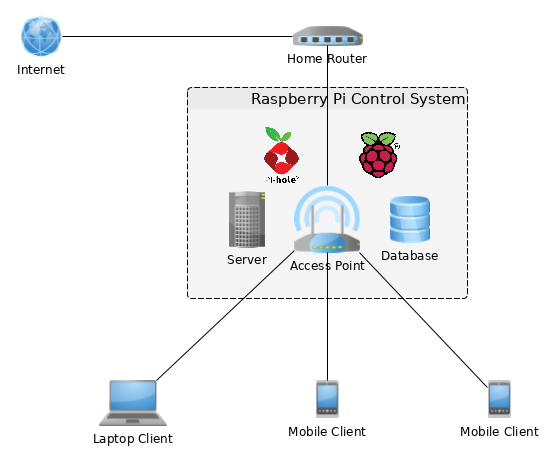
\includegraphics[width=1\textwidth]{Figures/system-diagram}
\decoRule
\caption{Raspberry Pi based parental control system diagram}
\label{fig:system-diagram}
\end{figure}

Another difference between out approach and the Circle device is that the core of system is built around the  Domain Name System, by using a local DNS server for filtering and blocking. For this test we are using the open source project Pi-hole, which uses the DNS forwarder and DHCP server Dnsmasq to create the blocking and filtering system, which serves the primary scope of blocking all ads. The framework used to develop the mobile application is Flutter \citep{flutterio}, an open-source mobile application development SDK created by Google, to make the mobile control application available on both Android and iOS. We also used the Netfilter framework for more fine control on the network traffic on the access point. The tools and technologies used are as follows:

\begin{itemize}
\item Raspberry Pi 3 - as the access point and main controller
\item Pi-hole - for blocking and filtering
\item Dnsmasq - as DNS forwarder
\item Netfilter - to control the traffic on the access point
\item Go lang - the create a REST server for the mobile application
\item Flutter - to implement the cross-platform mobile application
\end{itemize}

We will next present the principles behind each of these components of the system and details about how they all work together to make the parental control task easy for the parents and beneficial for children development.

\section{Raspberry Pi}

Raspberry Pi is a series of small single-board computers developed in the United Kingdom by the Raspberry Pi Foundation to promote the teaching of basic computer science in schools and in developing countries \citep{cellan2011raspberryPi}. All models feature a Broadcom system on chip (SoC) with an integrated ARM compatible central processing unit (CPU) and on-chip graphics processing unit (GPU). The model that we used for our setup is a Raspberry Pi 3 Model B, released in February 2016 with a 64 bit quad core processor and on-board WiFi, Bluetooth and USB capabilities. The presence of on-board WiFi card makes it suitable to run as an access point, the computing power is enough to run the setup that we need, the DNS forwarder and other tools. It also offers a rich software package, with multiple Linux-based operating system to choose from, the recommended version being Raspbian, a Debian-based system, which we use in our setup. The software community around the Raspberry Pi boards is also very active, which helps a lot in development and in troubleshooting any problems along the way. The Pi-hole system that we integrated into our system was also developed by the same community and created the opportunity for us to take it a step further and extend it by integrating the parental control features into it. We use the Raspberry Pi board as a wireless access point and also as a backend for the control system, since it is powerful enough to run the systems that we need. Out backend system has 4 main components: the Go server, the SQLite database, the Dnsmasq DNS forwarder and Pi-hole ad-blocking system, along with the quiz-taking system that we integrate, which is built using Ruby on Rails.

\section{Pi-hole}

Pi-hole is an Linux application which block advertisements and Internet trackers at the network-level, by acting as a DNS sinkhole, and also DHCP server, on a private network. A DNS sinkhole is the name gives to a DNS server that gives out false information to prevent the use of a certain domain name. It was designed for use on embedded devices with network capabilities, such as the Raspberry Pi. It has the ability to block traditional adverts on websites, but also adverts in other places, such as smart TVs and mobile operating systems. It works by serving as a DNS server for a private network and using a list of advert and tracking domains from predefined sources that the system uses to compare DNS queries to \citep{salmela2015pihole}. If a match is found in one of the block lists, Pi-hole will refuse to resolve the requested domain. This feature can be used to block any domains, not the advertisement ones, by extending the block list. 

We use this feature to block domains that are not considered useful for a child, such as social media platforms. You can also manually whitelist a domain, such that it is never blocked, and you can use the Pi-hole system to view reports about the DNS queries done by the clients. The main domain blocking feature works for all the clients, regardless of the age bracket, but we can establish certain domains for each age bracket that take priority in the visited domains reports. This approach is less restrictive for certain domains that are not bad, but does not bring much value for children either. We want the parent to know if the child spends to much time on these domains and to encourage discussion to find more valuable way of spending time online.

\subsection{How it works}

Pi-hole acts as a forwarding DNS server, so if it does not know where a domain is it forwards the query to another server. When you configure it, it knows where the ad-serving domains are, because they are all in the local list, along with all the explicitly blocked domains, so it does not have to forward those requests. But it does not know where the legitimate domains are, so those requests are forwarded to an upstream, recursive server. Those servers also don't know where it is only if they were asked to find it before, the only DNS servers that truly know where a domain is are the authoritative DNS servers. The flow of events that are triggered when Pi-hole receives a DNS query can be seen in the Figure \ref{fig:pihole-dns} \citep{salmela2017ftldns}.

\begin{figure}[th]
\centering
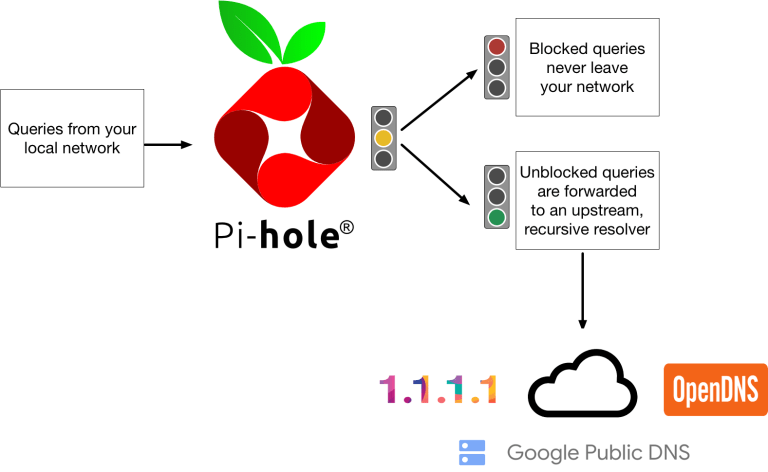
\includegraphics[width=1\textwidth]{Figures/pihole-dns}
\decoRule
\caption{The flow of traffic through the Pi-hole system}
\label{fig:pihole-dns}
\end{figure}

The flow of traffic goes like this:
\begin{enumerate}
\item The client asks the Pi-hole who is pi-hole.net
\item Pi-hole will check the cache and reply if the entry is present in the cache
\item Pi-hole will check the blocking list and if the domain is blocked, it will replay accordingly
\item If neither 2 or 3 are true, Pi-hole forwards the request to the external upstream DNS server, that was configured on installation
\item After receiving the answer from the upstream server, Pi-hole will reply to the client
\item Pi-hole save the answer in the cache to be able to respond more quickly if the same domain is queried again
\end{enumerate}

Pi-hole can also act as a network monitoring tool, since it logs all DNS queries sent to it, by default, so you can find what kind of traffic is going through your network. We integrated a component for visualizing this data into our system, to be able to quickly tell what domains are most visited by the children and what blocked domains they are trying to access. This integration was made easier by the fact that Pi-hole has a component which takes the raw data from the logs and pre-process it, storing it in a local database, to be able to serve quickly the types of queries needed, such as the top visited domains and the top blocked domains. We access this data by using a socket and some predefined commands. Pi-hole offers also a web interface to view these detailed reports. You can see the query types over time, forward destination over time, top domains, top blocked domains and other useful reports, as can be seen in the Figure \ref{fig:pihole-admin}.

\begin{figure}[th]
\centering
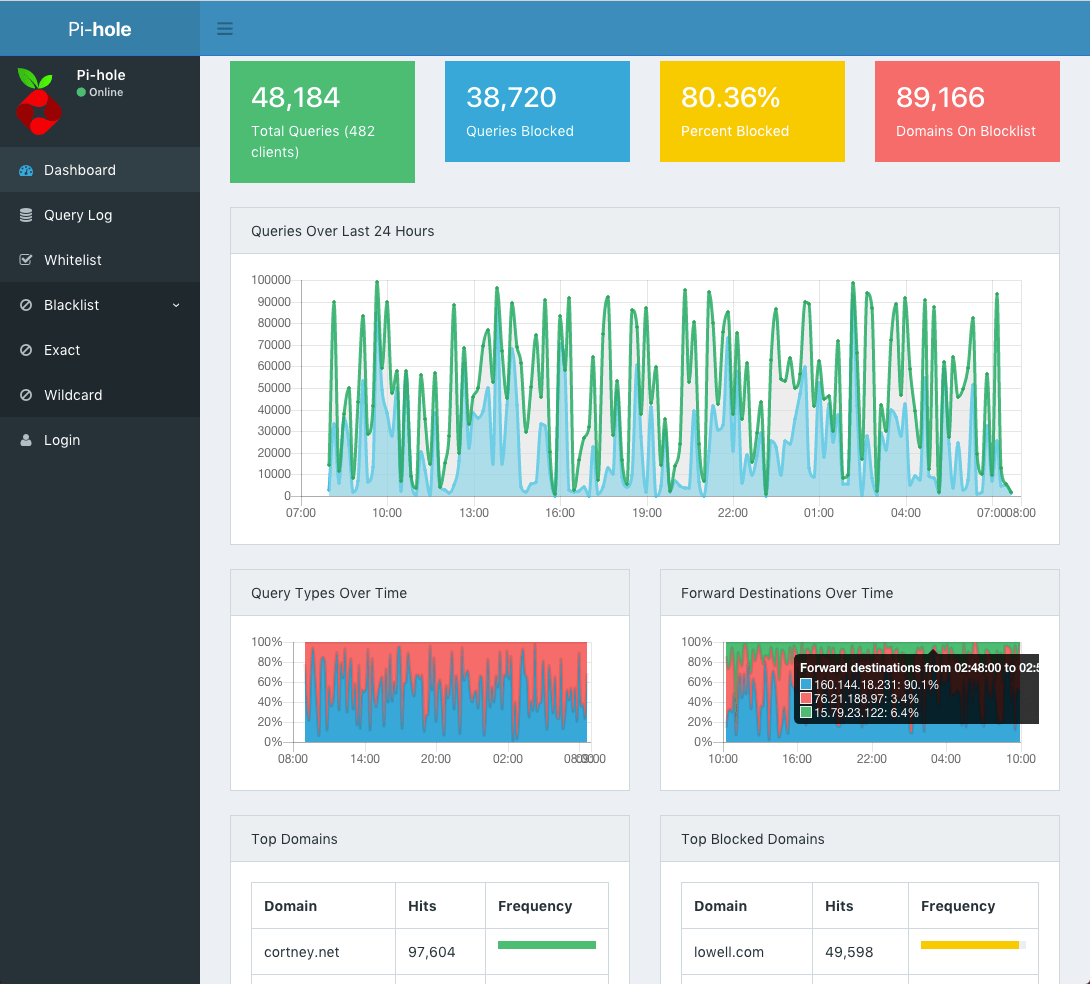
\includegraphics[width=1\textwidth]{Figures/pihole-admin}
\decoRule
\caption{The Pi-hole admin dashboard}
\label{fig:pihole-admin}
\end{figure}

Other benefits that Pi-hole brings to your local network are related to bandwidth and network speed. Because it works at the DNS level and prevents the ads and blocked domains from being downloaded. Since these ad images, videos and sounds are not being downloaded, the network will perform better. For the same reasons, it also reduces bandwidth, by preventing undesired assets from being downloaded. You can also extend the default block list to include sites that are known to serve malware or act as a phishing site, which brings another level of security, very important in the context of children using the Internet. The performance should not be a problem for the Pi-hole system, since even a not so powerful Raspberry Pi has been documented of handling up to 60 clients without problems, more than enough for a family network \citep{salmela20177things}.

\section{Dnsmasq}

Dnsmasq is a lightweight and easy to configure DNS forwarder and DHCP server. It can be used to serve names for local machines which are not in the global DNS and is designed to offer DNS and DHCP solutions for small networks \citep{debianHowToDnsmasq}.
It has low resource requirements for system resources, so it is a good solution for our Raspberry Pi setup. It improves the performance and reduces the load on upstream DNS servers by caching DNS records locally.

Dnsmasq loads the content of /etc/hosts file to be able to resolve local names, and that allows some useful tricks, such as overriding some global domains, by adding a line with the format "0.0.0.0 annoyingsite.com". This prevents the domain annoyingsite.com from being resolved and that's the way Pi-hole uses it to block ads, by creating an entry for each known ad serving domain, and we also use that to block any other unwanted domains. Pi-hole keeps this Dnsmasq related configuration in a file named gravity.list, which is updated periodically to include the newest ad domains. It currently contains around 126000 of ad domains and the number is constantly growing. We can see below some of the line from this files, with 10 blocked ad serving domains.

\begin{lstlisting}
192.168.0.103 zxypenguin.people-group.su
192.168.0.103 zy.zeroredirect1.com
192.168.0.103 zyban-store.shengen.ru
192.168.0.103 zyban.1.p2l.info
192.168.0.103 zyban.about-tabs.com
192.168.0.103 zybezradio.com
192.168.0.103 zyiztazhfprochain.review
192.168.0.103 zyjyyy.com
192.168.0.103 zyngatables.com
192.168.0.103 zyngawithfriends.com
\end{lstlisting}

The included DHCP server functionality supports static and dynamic DHCP leases, multiple networks and IP address ranges. We define a DHCP range for our network, along with the upstream DNS servers to use. The defined upstream DNS servers are the Google one and the configuration for this looks as follows:

\begin{lstlisting}
server=8.8.8.8
server=8.8.4.4
interface=wlan0
dhcp-range=10.0.0.2,10.0.0.5,255.255.255.0,12h
\end{lstlisting}

Other Dnsmasq feature that is for use for us is that it can support different DNS server configuration for different DHCP settings. We are using this to establish the way the two classes of users defined in out system can access the network, since we don't want to apply the same blocking rules for the parents as for the children. Dnsmasq supports defining a different DNS resolver based on MAC address, and we use that to allow the parent's device to bypass the domain blocking rules that apply only to children devices, by configuring the system to use the Google resolver for that devices. That is easily done by adding the following rules to the Dnsmasq configuration:

\begin{lstlisting}
## This will go straight to Googles DNS Servers.
dhcp-option=tag:googlesdns1,6,8.8.8.8
dhcp-option=tag:googlesdns2,6,8.8.4.4

## This will go straight to Opendns Servers.
dhcp-option=tag:opendns1,6,208.67.222.220
dhcp-option=tag:opendns2,6,208.67.222.222

## Your Device that goes to Google DNS
#dhcp-host=dc:0b:34:cc:b0:ff,set:googlesdns1 #Nexus

## Your Device that goes to OpenDNS
#dhcp-host=a8:b8:6e:41:0e:de,set:opendns1
#dhcp-host=f8:23:b2:ad:4d:f3,set:opendns1
\end{lstlisting}

We can configure different devices to work with different DNS servers, to add another level of control over the blocking features \cite{archwikiDnsmasq}.

We are using the DHCP server functionality of Dnsmasq, to have control over what IP address gets every device and to easily identify the client devices by MAC and IP address, to be able to interpret the query logs and block access for specific devices. We establish a DHCP range for the clients of the access point, with a lease duration of 12h, but since all the logic works based on MAC address, the IP address is used only for display purposes. Because Dnsmasq is able to resolve local domains, we use that feature to block ad domains and other domains unsafe for children. To enable access for the parent's devices to the blocked domains, we use a configuration with a different DNS server, the Google one, for the admin devices.

\section{Netfilter}

The Netfilter framework \citep{netfilterorg} allows various networking-related operations implemented in the form of customized handlers and is provided by any Linux operating system. It offers various packet filtering, network address translation and port translation features to provide the functionality required for directing packets through a network and also block packets from reaching certain locations within the network. Netfilter is represented by a set of hooks inside the Linux kernel which allows the registration of callback functions for specific kernel modules. These functions are applied as filtering and modification rules and are called for each packet that traverses the respective hook in the networking stack.

The most significant parts of the Netfilter hook system are the modules named ip\_tables, ip6\_tables and arp\_tables. They provide a firewall system based on rules that can filter or transform packets. These rules are organized into tables which classify them according to the type of decision they are used to make. For example, there are rules dealing with network address translation and rules dealing with the decision to allow a packet to continue to its destination or not. The tables that iptables provides are \citep{ellingwood2015iptables}:

\begin{itemize}
\item filter table, used to make decisions whether a packet should be allow or not to reach its destination
\item NAT table, used to implement network address translation rules, to determine if and how to modify the packet's source or destination address
\item mangle table, used to alter the packet headers in different ways, such as adjusting the TTL (Time to Live) value
\item raw table, with the purpose of marking packets in order to opt-out of connection tracking features built on top of the Netfilter framework
\item security table, used to set internal SELinux security context marks on packets
\end{itemize}

Within each table, the rules are organized into separate chains, which corresponds to the Netfilter hooks that trigger them. The names of the built-in chains, with the corresponding hook, are \citep{ellingwood2015iptables}:

\begin{itemize}
\item PREROUTING, triggered by the NF\_IP\_PRE\_ROUTING hook by any incoming traffic as soon as entering the network stack.
\item INPUT, triggered by the NF\_IP\_LOCAL\_IN hook after the incoming packet has been routed if destined for the local system
\item FORWARD, triggered by the NF\_IP\_FORWARD hook after the incoming packet has been routed if it is to be forwarded to another host
\item OUTPUT, triggered by the NF\_IP\_LOCAL\_OUT hook by any outbound traffic created locally when it hits the network stack
\item POSTROUTING, triggered by the NF\_IP\_POST\_ROUTING hook after routing and before sending the traffic out on the wire
\end{itemize}

The complex flow of a packet through the Netfilter framework can be seen in the Figure \ref{fig:netfilter-flow}, with all the layers and tables involved.

After configuring the Raspberry Pi to work as a wireless access point \citep{raspberryPiAccessPoint} by using the user space daemon hostapd \citep{hostapd}, we have to enable IP forwarding for the wireless clients, such that they are able to access the Internet, not just the local network.  This is done by changing the following setting in the /etc/sysctl.conf file:

\begin{lstlisting}
net.ipv4.ip_forward=1
\end{lstlisting}

We need to also add a new rule for the outbound traffic on the eth0 interface, which provides the Internet connection to the Raspberry Pi. This is done by adding a POSTROUTING rule to mask the private IP address of a node with the external IP address of the gateway, using the MASQUERADE target: 

\begin{lstlisting}
sudo iptables -t nat -A  POSTROUTING -o eth0 -j MASQUERADE
\end{lstlisting}

To give Internet access to the access point clients connected on the wlan0 interface we have to add the following filter FORWARD rule:

\begin{lstlisting}
sudo iptables -A FORWARD -i eth0 -o wlan0 -m state --state RELATED,ESTABLISHED -j ACCEPT
\end{lstlisting}

We also use iptables rules to allow or block all network access for specific devices and to enforce the time limits for them. To block access for a device we add an INPUT rule for a device with a specific MAC address to drop the packets, by running the command like:

\begin{lstlisting}
sudo iptables -A INPUT -i wlan0 -m mac --mac-source 3C:83:75:D0:DA:C4 -j DROP
\end{lstlisting}

To allow back access for the blocked device, we run the command to remove the rule:

\begin{lstlisting}
sudo iptables -D INPUT -i wlan0 -m mac --mac-source 3C:83:75:D0:DA:C4 -j DROP
\end{lstlisting}

These commands are also run by the Go back-end using a cron table, to enforce time limits for network access for devices.

\begin{figure}[th]
\centering
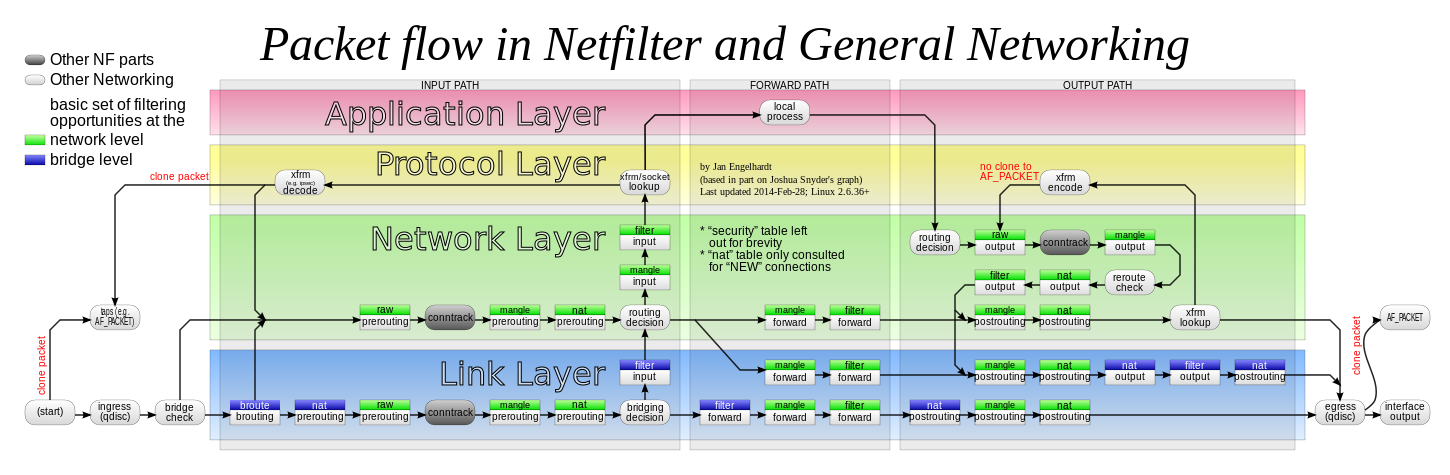
\includegraphics[width=1\textwidth]{Figures/netfilter-flow}
\decoRule
\caption{Flow of network packets through the Netfilter}
\label{fig:netfilter-flow}
\end{figure}

\section{Mobile application}

In order to give the parents easy access on the network rules that the system support, we developed a mobile application.
Using the application, a parent can easily establish the supported content control rules and view a short summary of usage for each device. The application has a simple client-server architecture, using a Go-lang back-end running on the Raspberry Pi and a cross platform mobile application, running on Android and iOS devices. The data needed to configure the system is minimal, so we used the relational database management system SQLite \citep{sqlite}, since it is easily configurable and does not require powerful hardware to run on, which makes it suitable for the Raspberry Pi. 


\subsection{Database}
Since not much data is needed for the system to work, the database diagram is fairly simple, as we can see in the Figure \ref{fig:database-diagram}. The most important entries are the users, which represents a child, and the association between a user the the devices it owns. Each device is represented by the state it is in, blocked or not, and the time frame that if has access to the Internet. Each user corresponds to an age bracket, if it does not have the admin flag set. The age bracket is linked to a set of the blocked domains and this relation is used when showing the usage summary for each device, to establish a higher priority for the associated domains. This is used when the domains from the list are not blocked, in order to give the parent an idea about how much each child uses the domains that are considered not useful for its age and to initiate a discussion about this.

\begin{figure}[th]
\centering
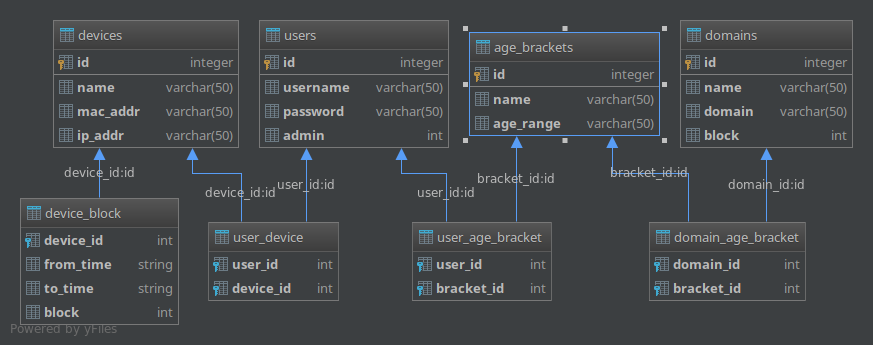
\includegraphics[width=1\textwidth]{Figures/database-diagram}
\decoRule
\caption{Database diagram}
\label{fig:database-diagram}
\end{figure}

\subsection{Server}

The language of choice for the back-end system is Go \citep{golang}. Go is an open source programming language that makes it easy to build simple, reliable and efficient software. We chose this language because of its rich open source support, its powerful remote package management tools and the built-in concurrency primitives: light-weight processes (goroutines), channels and the select statement. This features provides a strong foundation for building a RESTful web service to run in a resource limited environment, like the Raspberry Pi. The rich open source support and libraries makes it easy to build such a system and quickly scale it.

At the root of our back-end system, we use the package gorrila/mux \citep{gorillaMux}, which implements a request router and dispatcher for matching incoming requests to their respective handler. This package makes it easy to define multiple routes, represented by a pattern in the URL, and their corresponding handlers. We defined a Route struct to hold the necessary parameters, such as URL pattern and handler, and we initialize the router using a list of Routes. Some of the routes that we define are:

\begin{lstlisting}[language=Golang]
Route{
	"Users",
	"GET",
	"/users/{userId}",
	usersHandler,
},
Route{
	"AddUser",
	"POST",
	"/add_user",
	addUserHandler,
},
Route{
	"Devices",
	"GET",
	"/devices/{userId}",
	devicesHandler,
},
Route{
	"RegisterDevice",
	"POST",
	"/register_device/{userId}",
	registerDeviceHandler,
}
\end{lstlisting}

The router is created by a single command, and then the routes list is registered with the router, by adding the correspondig handler to each pattern:

\begin{lstlisting}[language=Golang]
router := mux.NewRouter()
for _, route := range routes {
	router.Handle(route.Pattern, 
		jwtMiddleware.Handler(route.HandlerFunc)).
		Methods(route.Method)
}
\end{lstlisting}

Mux supports the addition of middlewares to a Router, which are executed in the order they are added if a match is found, including its subrouters. Middlewares are (typically) small pieces of code which take one request, do something with it, and pass it down to another middleware or the final handler. Some common use cases for middleware are request logging, header manipulation. We use that to add a JSON Web Token (JWT) \citep{rfcJWT} middleware to the router, in order to be able to use an JWT as an access token to our API, such that only our mobile client can make requests. JWT is a compact, URL-safe means of representing claims to be transferred between two parties, and we use it to secure our API.

An example handler, which loads the domains defined in the system to support blocking and handles the /domains route, is:

\begin{lstlisting}[language=Golang]
func domainsHandler(w http.ResponseWriter, r *http.Request) {
	db, err := sql.Open("sqlite3", "./clients.db")
	checkError(err)
	defer db.Close()

	rows, err := db.Query("select d.id, d.name, d.domain, d.block from domains d")
	checkError(err)
	defer rows.Close()

	var netDomains Domains
	for rows.Next() {
		var id int
		var name string
		var domain string
		var block int

		err = rows.Scan(&id, &name, &domain, &block)
		checkError(err)
		fmt.Println(id, name, domain)
		domainElement := Domain{Id: id, Name: name, Domain: domain, Block: block}
		netDomains = append(netDomains, domainElement)
	}
	err = rows.Err()
	checkError(err)
	json.NewEncoder(w).Encode(netDomains)
	json.NewEncoder(os.Stdout).Encode(netDomains)
}
\end{lstlisting}

The back-end defines multiple router and handlers for them, in a way that corresponds to the routes we have on the clients side, so we will detail the routes and features in the next session.

Other packages used on the server side is JSON encoding package, because we use this open-standard file format to transfer data between the client and server, the SQLite integration package and the cron package, to implement the job runner that we need to establish the temporal Internet access rules.

\subsection{Client details}

We needed to make the parental control experience consistent on both major platforms, Android and iOS, and that's why we are using the mobile framework Flutter, a modern and cross-platform approach offered by Google. Flutter is open-source and is used for crafting high-quality native interfaces on iOS and Android. The development process is fast because of the rich set of fully-customizable widgets and the native performance is full because it incorporates all the critical platform differences.

The application UI is structured in a hierarchical manner. We have a high level menu with and entry for each main feature, like blocking and reporting. Under each main menu entry, we have multiple sub-menus corresponding to the related functionality. The navigation between different pages of the user interface is done using a router, which support query string parameter parsing and function handlers. We start by creating the router and other application configuration, and then navigating to the home page, different for a child or admin type user, but if the user is not logged in, it is presented with the log-in screen first. A list of routes, which we will detail in the following sections, can be seen in the listing below. These routes closely match the routes that we have defined on our REST web service, which is used to handle the client requests.

\begin{lstlisting}
static String root = "/";
static String adminRoute = "admin";
static String userHomeRoute = "userHome";
static String registerDeviceRoute = "register_device";
static String usersRoute = "users";
static String addUserRoute = "add_user";
static String devicesRoute = "devices";
static String deleteDeviceRoute = "delete_device";
static String addDeviceRoute = "add_device";
static String getDeviceBlockRoute = "get_device_block";
static String setDeviceBlockRoute = "set_device_block";
static String domainsRoute = "domains";
static String addDomainRoute = "add_domain";
static String editDomainRoute = "edit_domain";
static String deleteDomainRoute = "delete_domain";
static String topDevicesRoute = "top_devices";
static String topDomainsRoute = "top_domains";
\end{lstlisting}

The navigation to a new route is done by calling navigateTo on the router object, with the context and the route pattern, including parameters, as arguments. We can see in the listing below how we navigate to the devices view for a user, by using the user ID as parameter to the route pattern:

\begin{lstlisting}
router.navigateTo(context, "${Routes.devicesRoute}?userId=${user.id}");
\end{lstlisting}

For the user interface component, we build custom widgets by extending the StatefulWidget class to create lists, cards or forms that fits our model elements and hold state that we need for the application to work, such as domain or device blocking state. In the listing below we can see how we build a scrollable list view by loading all the devices for the a user, and the resulting UI component in Figure \ref{fig:user-devices}. The block icon on the right represent the state of the device, blocked or not, and that state changes on list item tap.

\begin{lstlisting}
class DevicesWidget extends StatefulWidget {

  final int userId;

  DevicesWidget(this.userId);

  @override
  State createState() {
    return new DevicesWidgetState(userId);
  }
}

class DevicesWidgetState extends State<DevicesWidget> {
  final _biggerFont = const TextStyle(fontSize: 18.0);
  final int userId;

  DevicesWidgetState(this.userId);

  Widget _buildDevicesList() {
    print("_buildDevicesList");

    RestDataSource restDataSource = new RestDataSource();
    final Future<Response> response = restDataSource.get("${Routes.devicesRoute}/$userId");

    return new FutureBuilder(
      future: response,
      builder: (BuildContext context, AsyncSnapshot<Response> snapshot) {
        if (snapshot.data != null) {
          try {
            print("Devices response data: ${snapshot.data.body}");
            final responseJson = json.decode(snapshot.data.body);
            return new ListView.builder(
                padding: const EdgeInsets.all(16.0),
                itemBuilder: (context, index) {
                  if (index < responseJson.length) {
                    print("Device $index : ${responseJson[index]}");
                    if (responseJson[index] != null) {
                      Device netDomain =
                          Device.fromJson(responseJson[index]);
                      return _buildRow(netDomain);
                    }
                  }
                });
          } catch (e) {
            return new Text("Error loading: " + e.toString());
          }
        } else {
          return new CircularProgressIndicator();
        }
      },
    );
  }

  Widget _buildRow(Device value) {
    return new DeviceWidget(value, userId);
  }

  addDevice() {
    var router = Config.getInstance().router;
    router.navigateTo(context, "${Routes.addDeviceRoute}?userId=$userId");
  }

  @override
  Widget build(BuildContext context) {
    print("Build DevicesWidgetState");
    return new Scaffold(
      appBar: new AppBar(
          title: new Text('Devices'),
          backgroundColor: Colors.black87,
          actions: [
            new IconButton(
              icon: new Icon(Icons.add),
              onPressed: () => addDevice(),
            ),
          ]
      ),
      body: _buildDevicesList(),
    );
  }
}
\end{lstlisting}

\begin{figure}[th]
\centering
\includegraphics[width=0.4\textwidth]{Figures/devices}
\decoRule
\caption{The devices view for a user}
\label{fig:user-devices}
\end{figure}

\subsection{Blocking and filtering}

We provide two levels of filtering, for devices in particular and for domains in general, that are applied to all devices. The device level blocking is managed using the user UI. When accessing the user UI, we can see a list of users for which the current user is admin. Each user is shown in a card like view, with the profile picture, user name and the associated age bracket. We can also add a new user, by using the add menu from the top right corner. This menu gets us to the add page, to fill the user details. The user views can be seen in Figure \ref{fig:user-views}.

\begin{figure}
\centering
\begin{subfigure}{.5\textwidth}
  \centering
  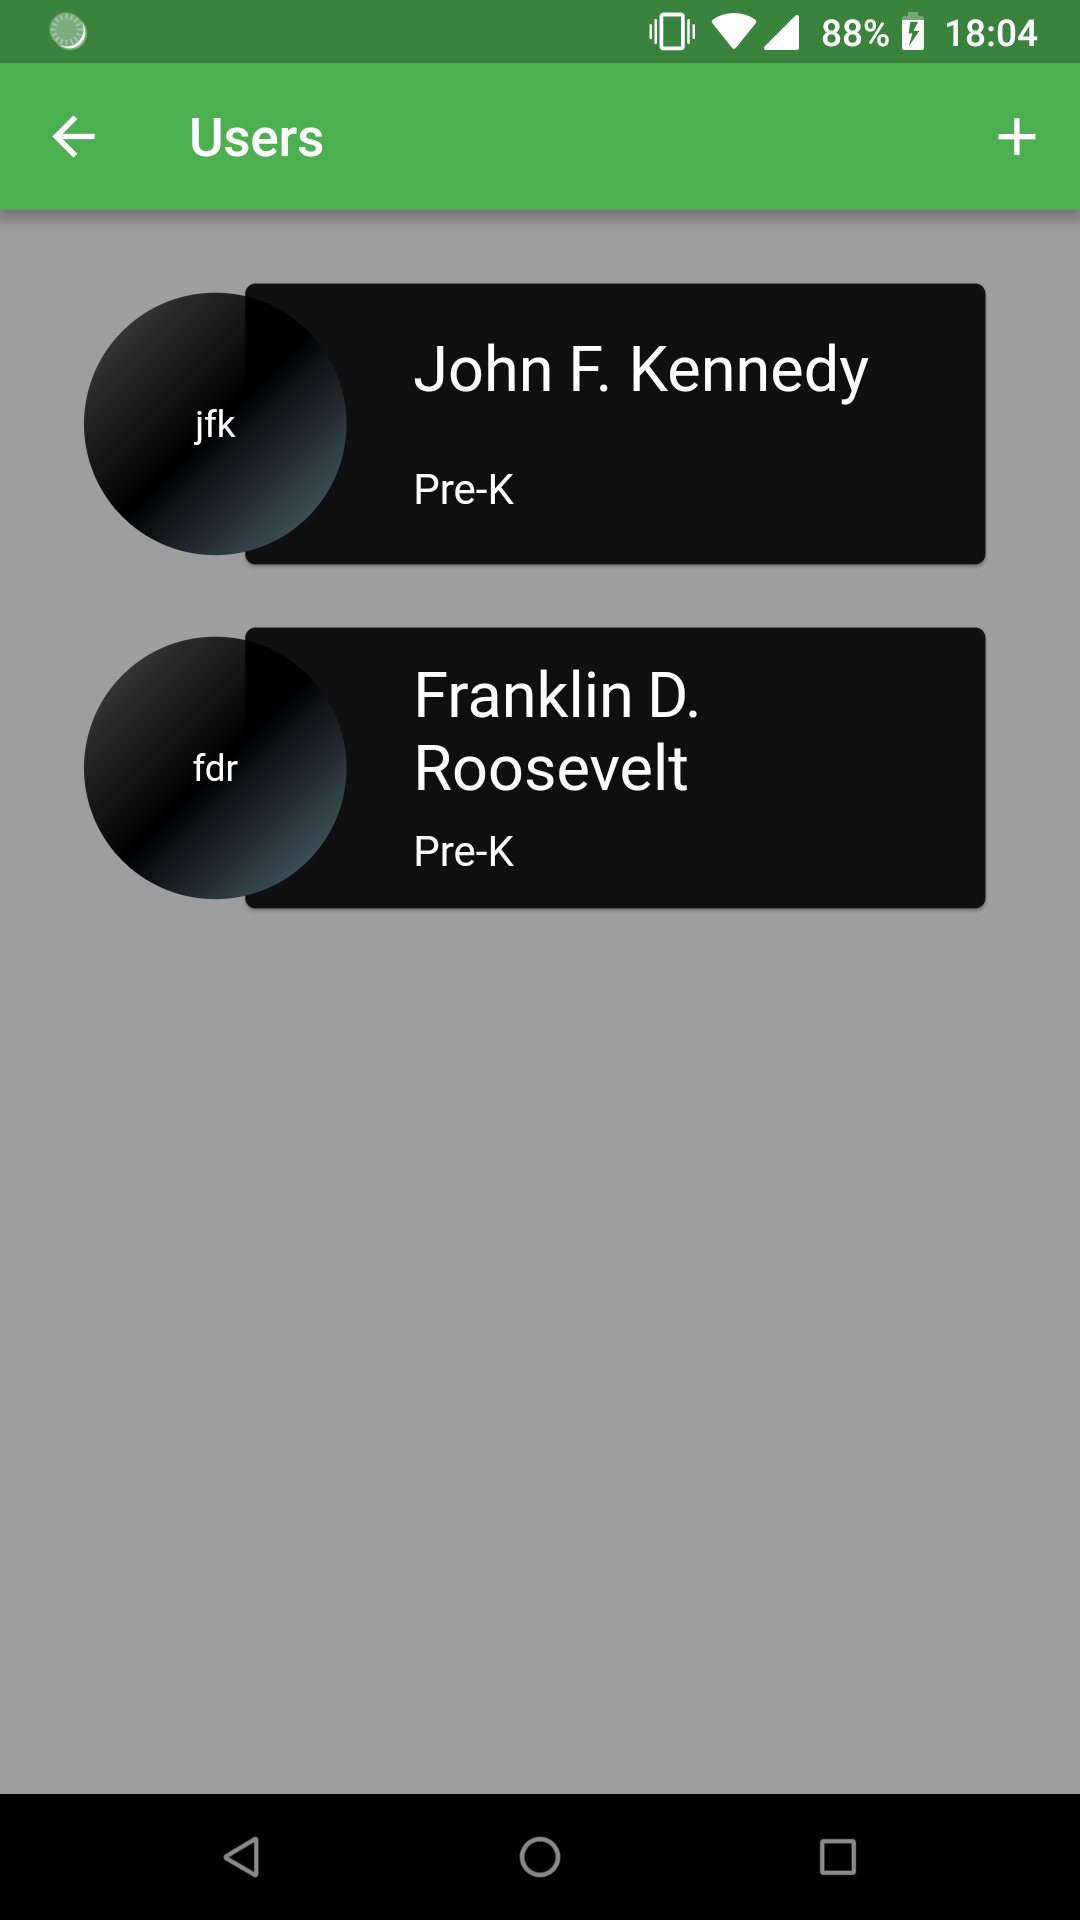
\includegraphics[width=.9\linewidth]{users}
  \caption{The user view}
  \label{fig:users}
\end{subfigure}%
\begin{subfigure}{.5\textwidth}
  \centering
  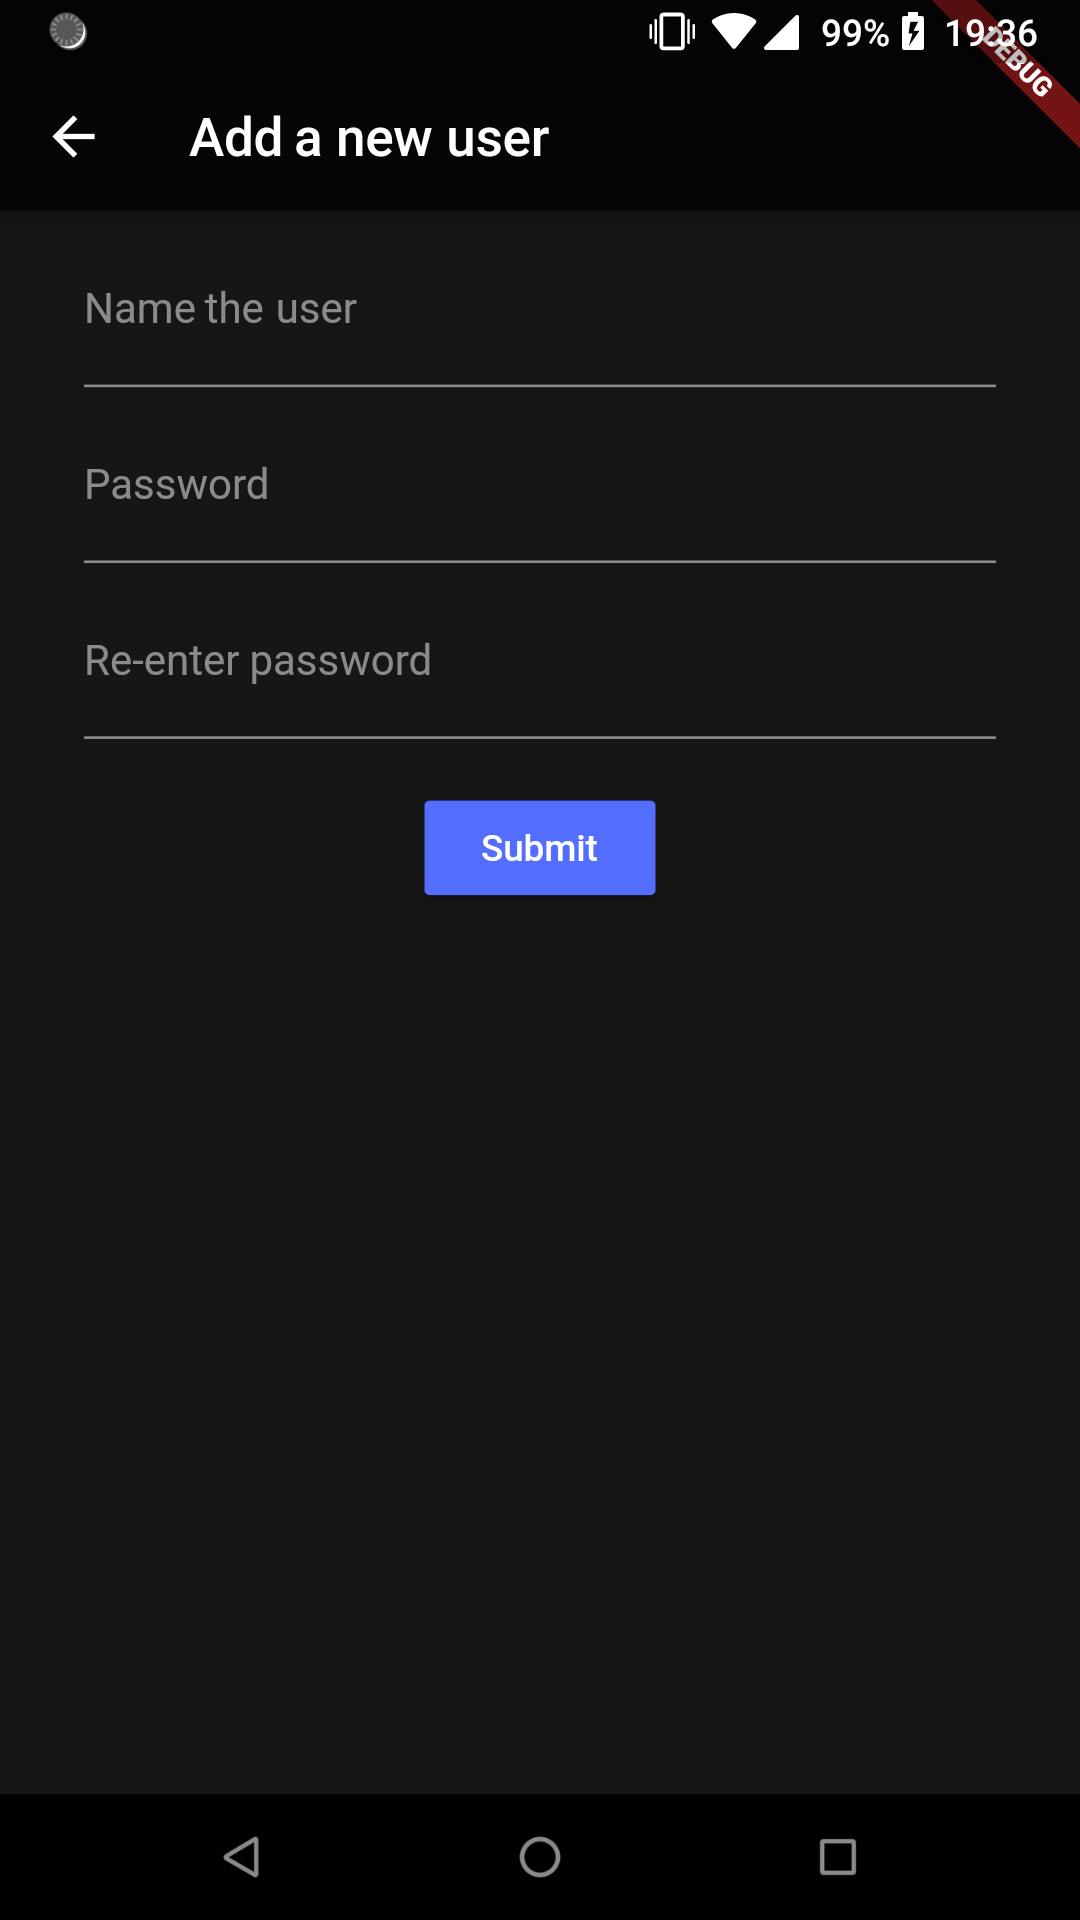
\includegraphics[width=.9\linewidth]{add-user}
  \caption{The add user view}
  \label{fig:add-user}
\end{subfigure}
\caption{The user related views}
\label{fig:user-views}
\end{figure}

For each user, we can view the list of associated devices by tapping on the user card. This gets us to a list of devices, which we can block or unblock, depending on the current state. A long press on a device shows a quick menu, from which we can access the time window setting component, where we can define the time interval in which the device has access to the Internet. That menu also allows the admin user to edit the details of a device or to delete it. We can also add a new device by using the top right menu item. All these view are shown in the Figure \ref{fig:device-views}.

\begin{figure}
\centering
\begin{subfigure}{.33\textwidth}
  \centering
  \includegraphics[width=.9\linewidth]{devices}
  \caption{The devices view}
  \label{fig:devices}
\end{subfigure}%
\begin{subfigure}{.33\textwidth}
  \centering
  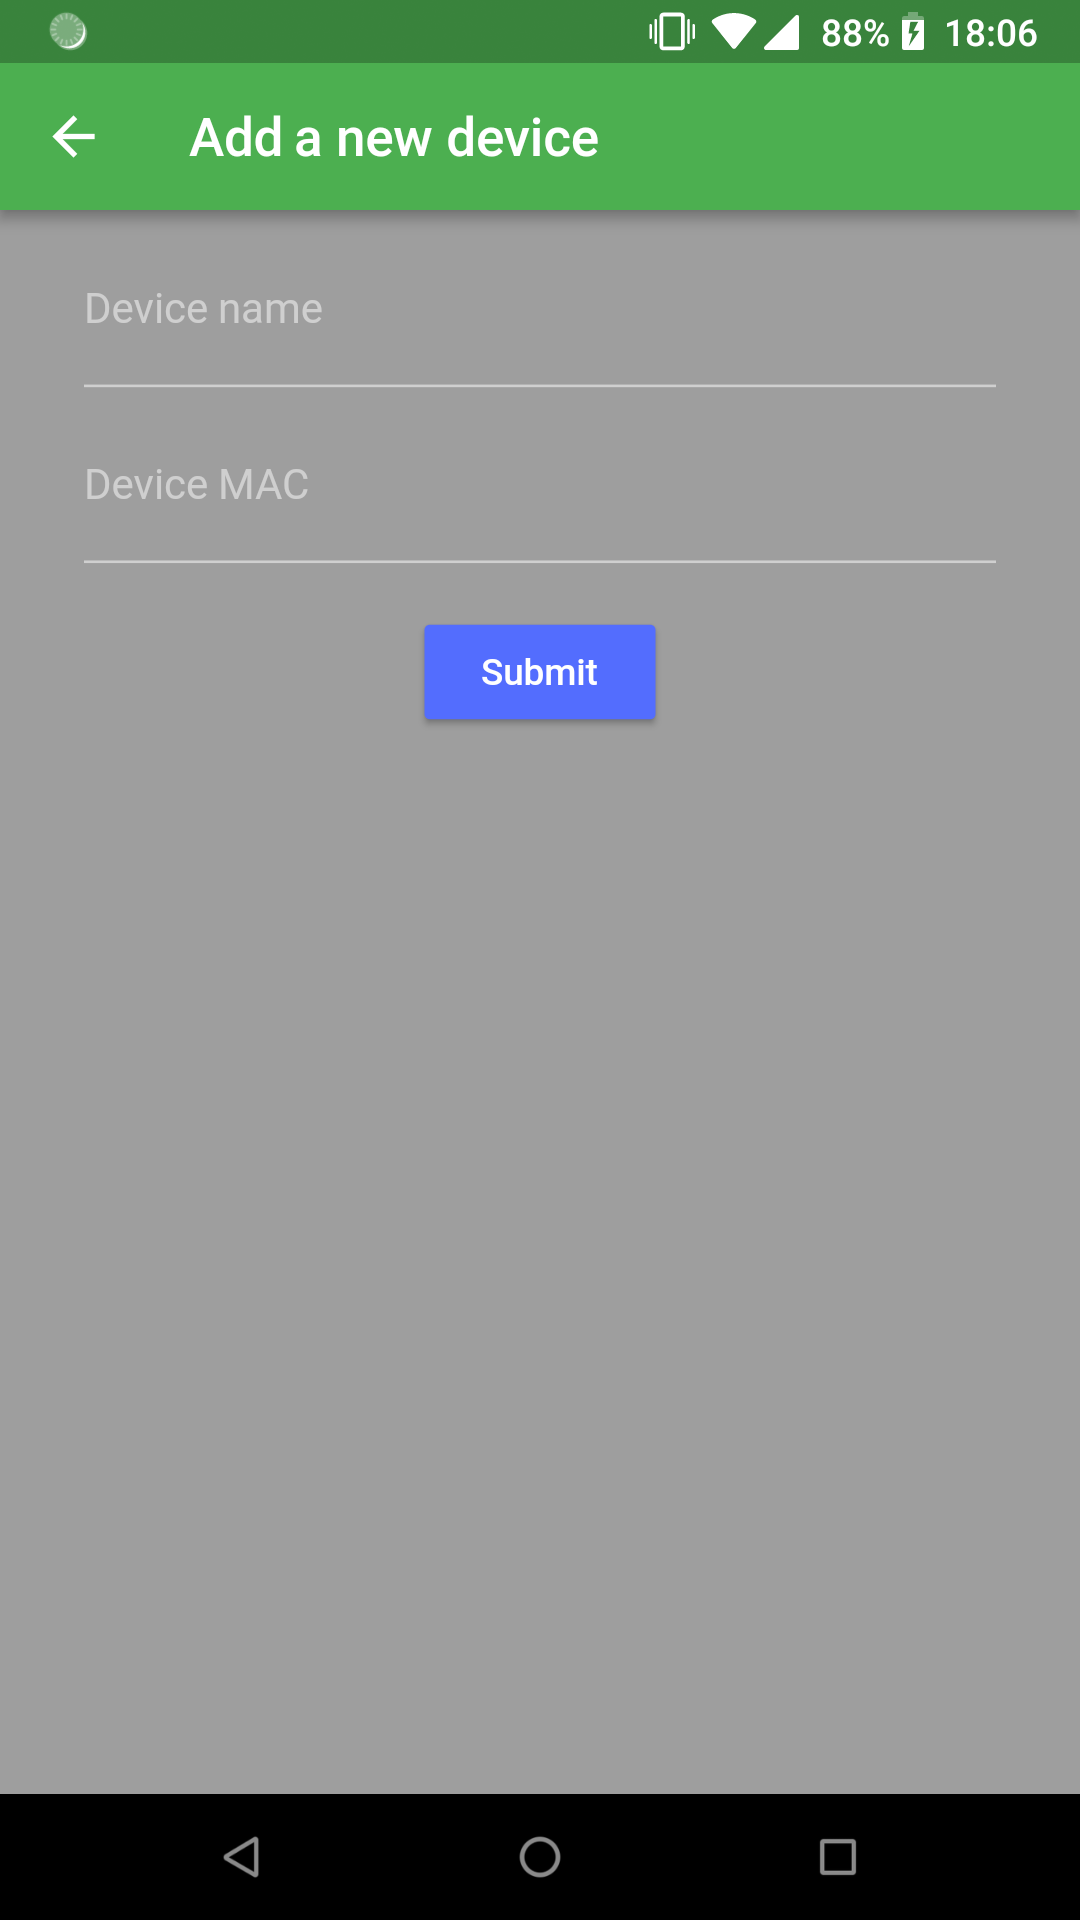
\includegraphics[width=.9\linewidth]{add-device}
  \caption{The add device view}
  \label{fig:add-device}
\end{subfigure}
\begin{subfigure}{.33\textwidth}
  \centering
  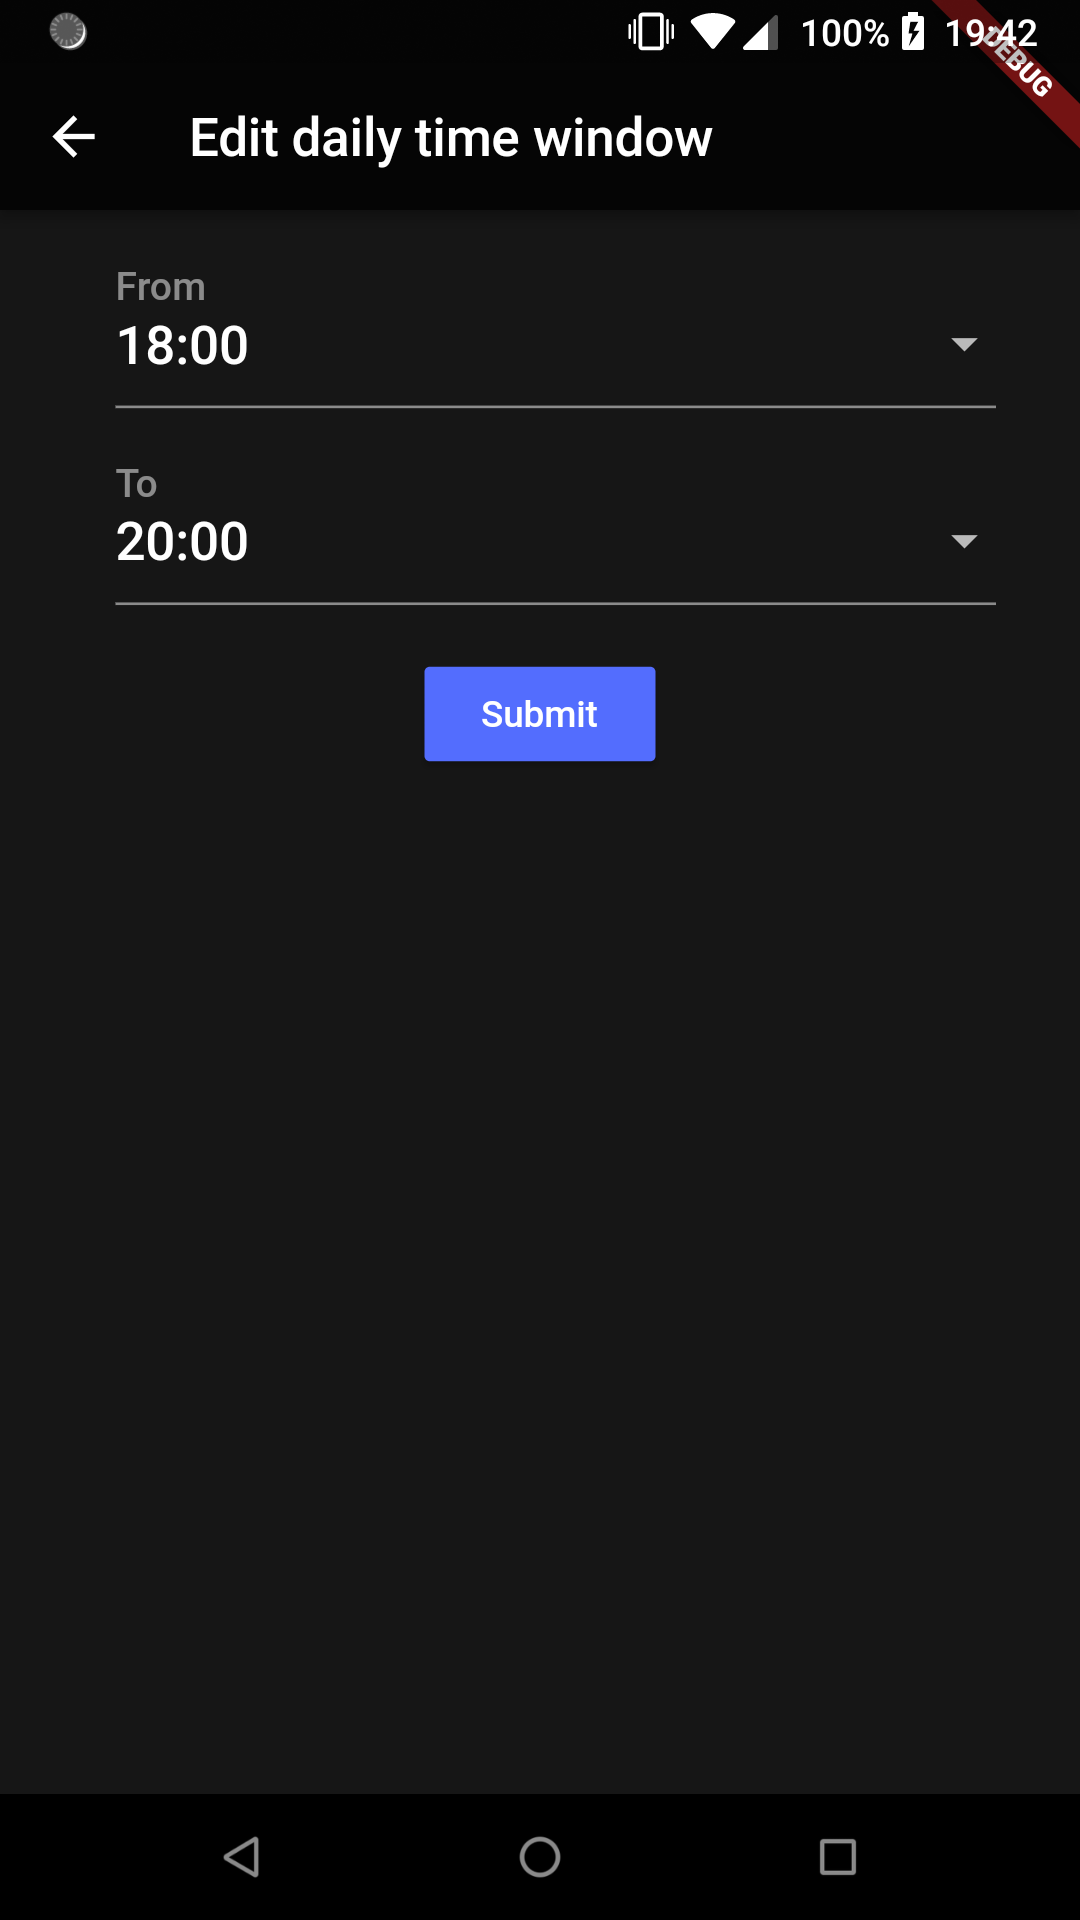
\includegraphics[width=.9\linewidth]{time-window}
  \caption{Device time window}
  \label{fig:time-window}
\end{subfigure}
\caption{The user related views}
\label{fig:device-views}
\end{figure}

\subsection{Reporting}

In contrast with the other parental control systems presented, we provide only limited reporting functionality, since we try to rely more on self-regulation than parental control. We try to encourage more communication between the parents and the children about Internet usage. The parent needs to understand some of the screen time usage of a child and he needs some data to get a starting point for the discussion. We try to provide this kind of data to the parent. This data is split into two categories: domains related query data and device related query data. The first category shows the top ten most visited domains, with the number of queries for each domains, while the second category show a top of devices with made the most requests to the DNS server. The related view tables can be seen in the Figure \ref{fig:top-views}.

\begin{figure}
\centering
\begin{subfigure}{.5\textwidth}
  \centering
  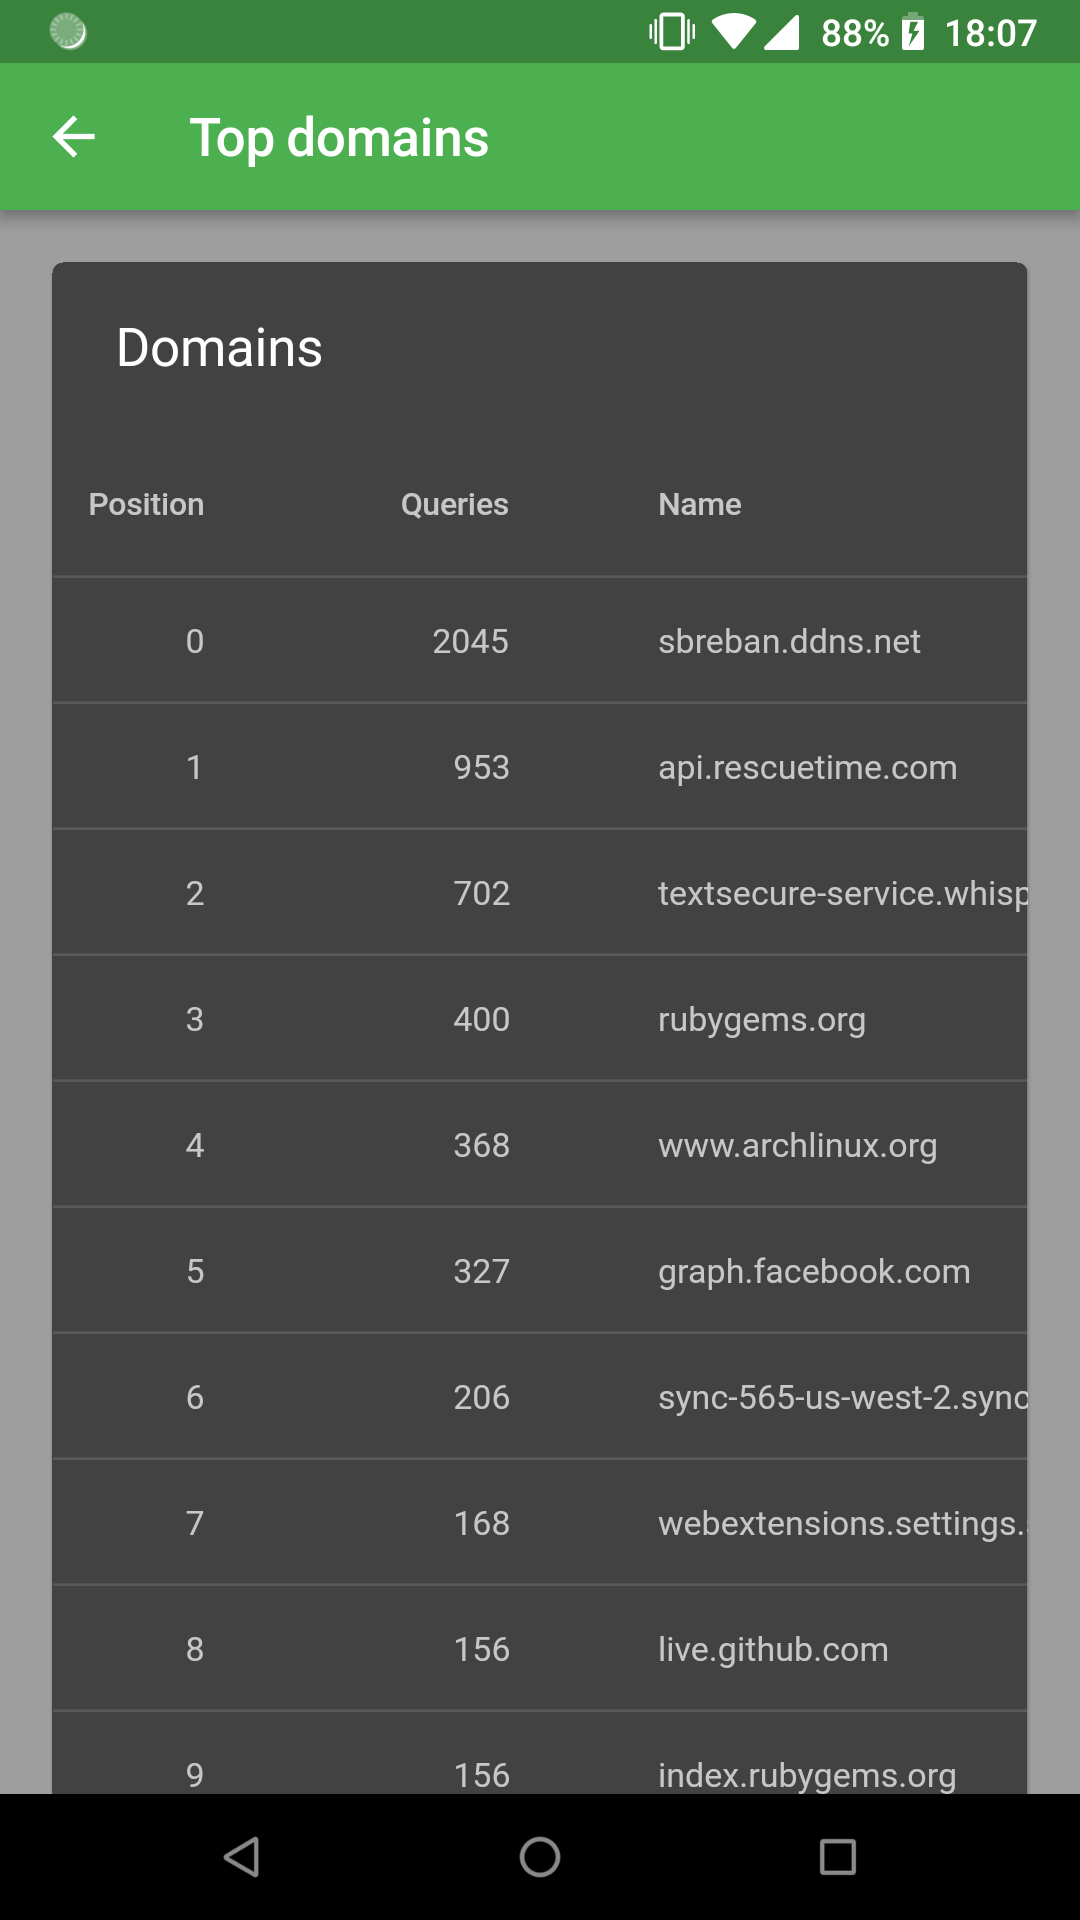
\includegraphics[width=.9\linewidth]{top-domains}
  \caption{Top domains view}
  \label{fig:top-domains}
\end{subfigure}%
\begin{subfigure}{.5\textwidth}
  \centering
  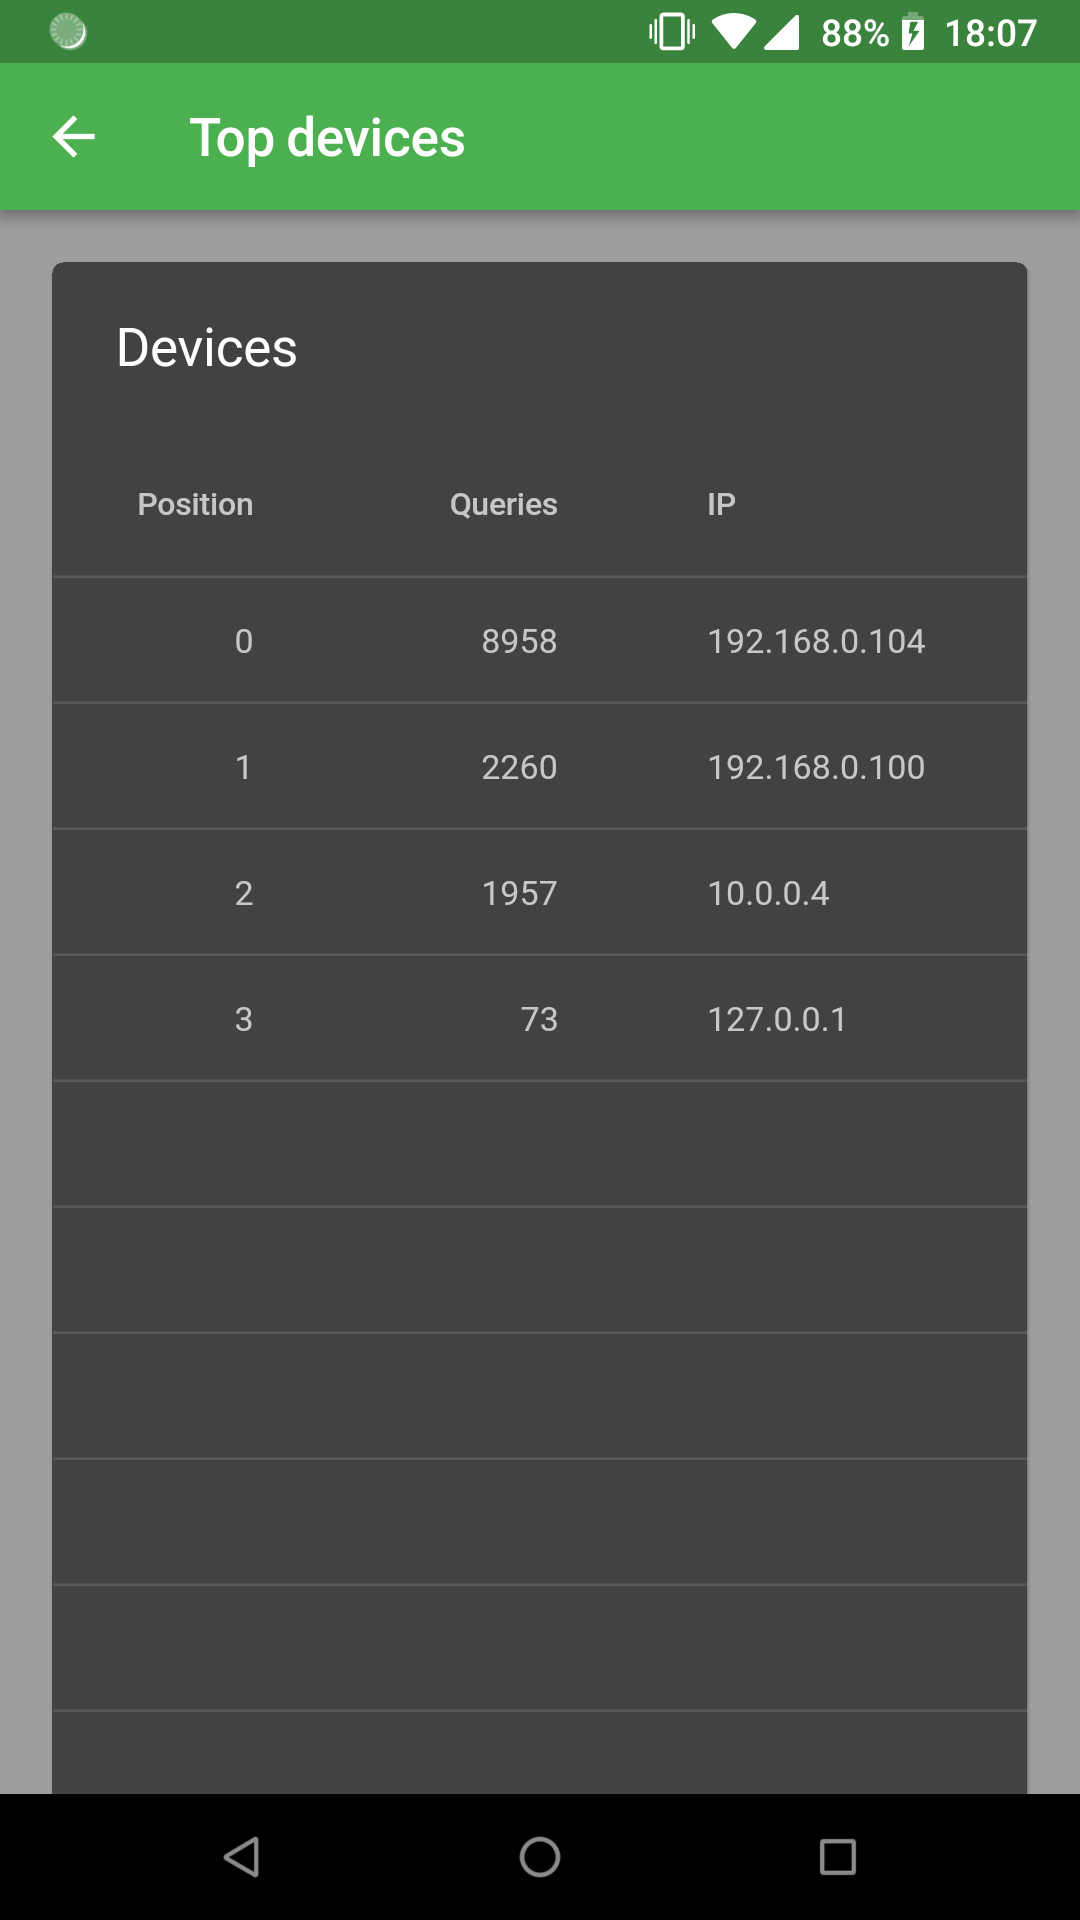
\includegraphics[width=.9\linewidth]{top-devices}
  \caption{Top devices view}
  \label{fig:top-devices}
\end{subfigure}
\caption{The reporting related views}
\label{fig:top-views}
\end{figure}

\section{Self regulation component}

\begin{figure}[th]
\centering
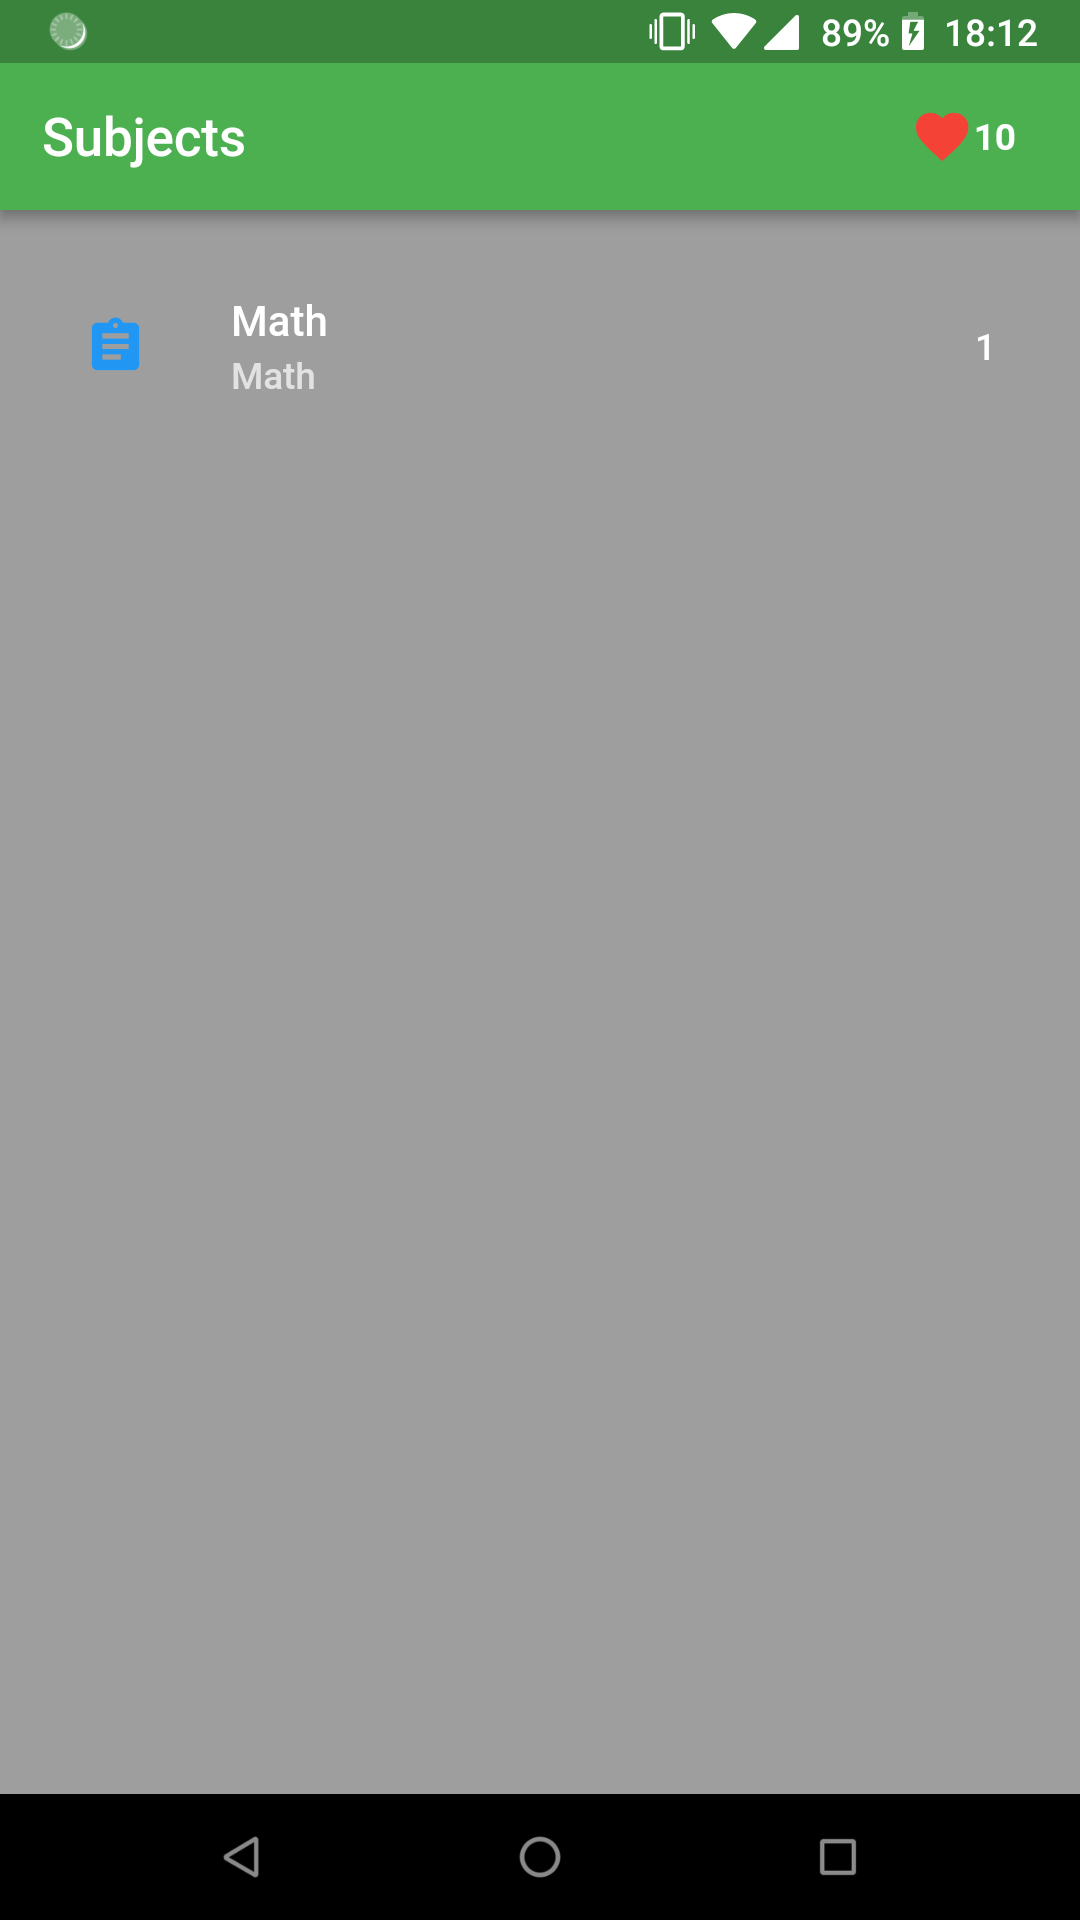
\includegraphics[width=0.4\textwidth]{Figures/subjects}
\decoRule
\caption{The subjects list view}
\label{fig:subjects}
\end{figure}

\begin{figure}
\centering
\begin{subfigure}{.5\textwidth}
  \centering
  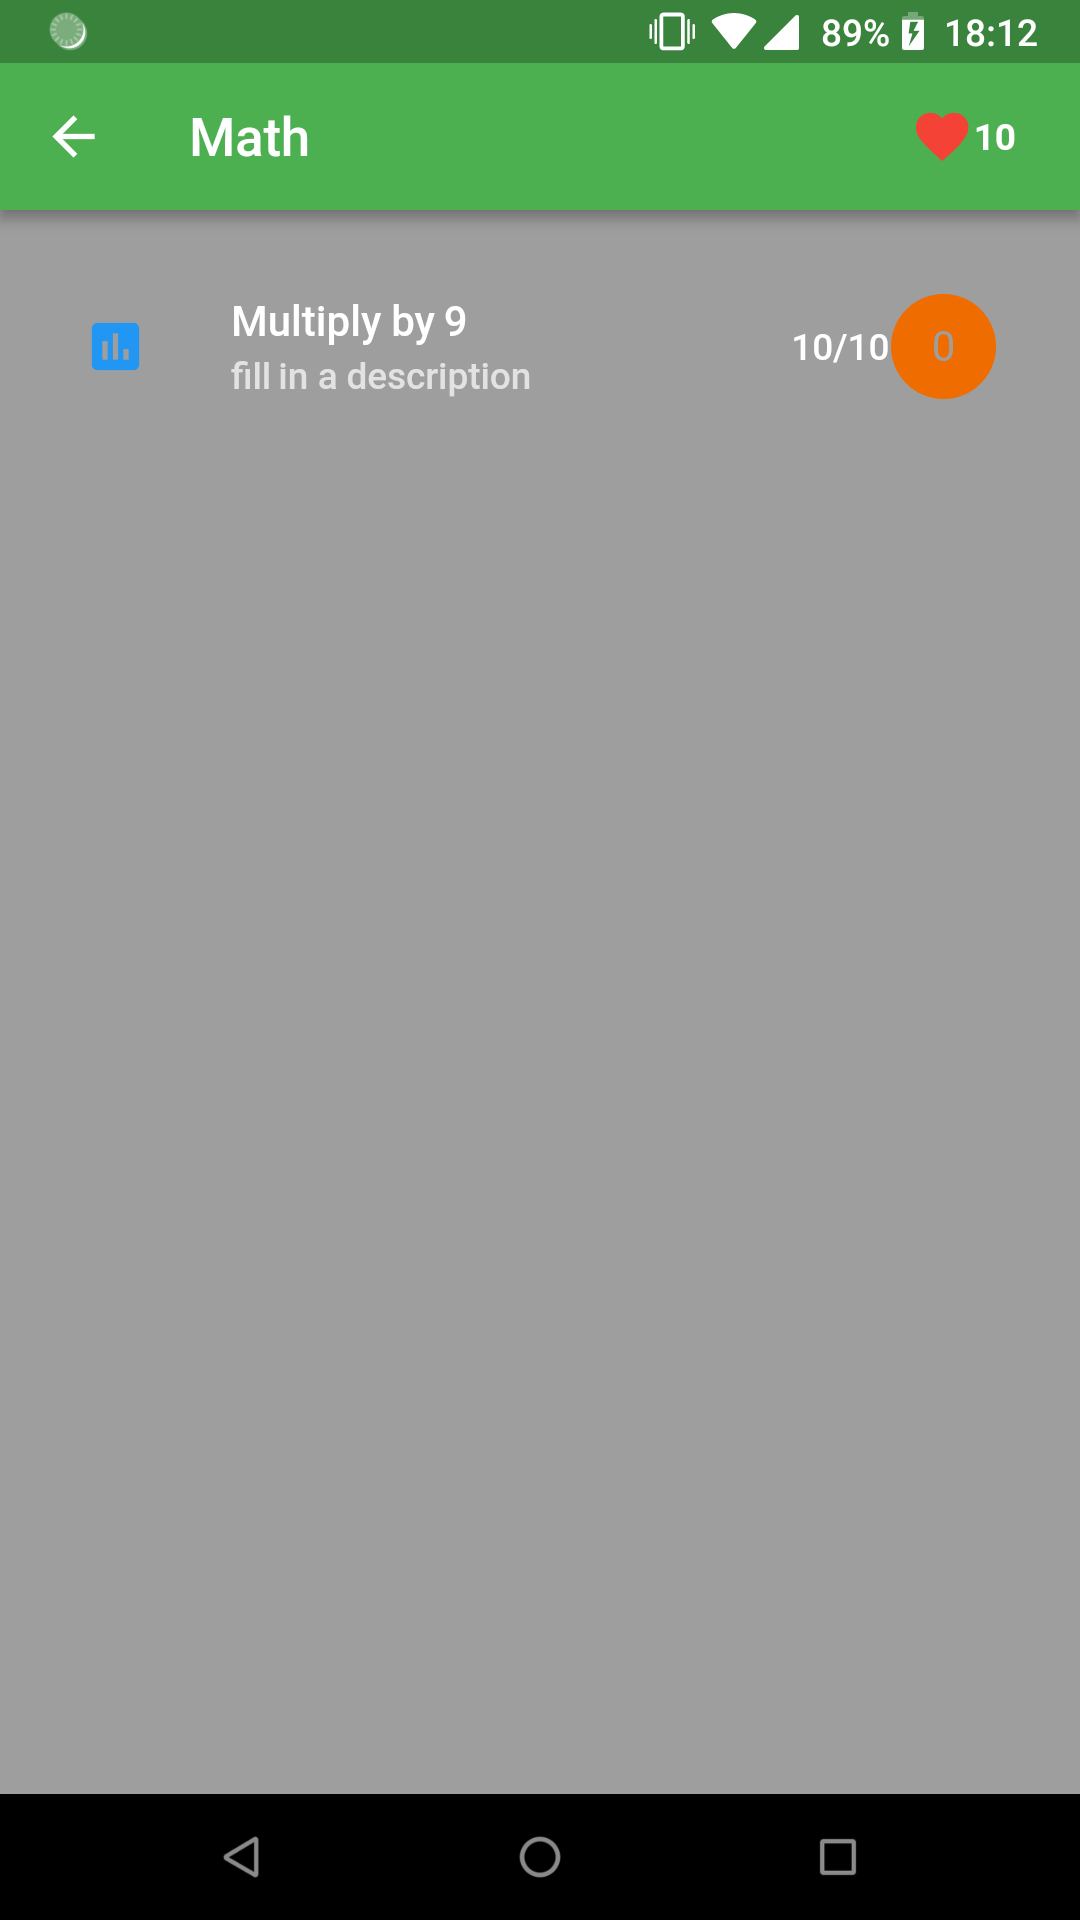
\includegraphics[width=.9\linewidth]{quizzes}
  \caption{The quizzes list view}
  \label{fig:quizzes}
\end{subfigure}%
\begin{subfigure}{.5\textwidth}
  \centering
  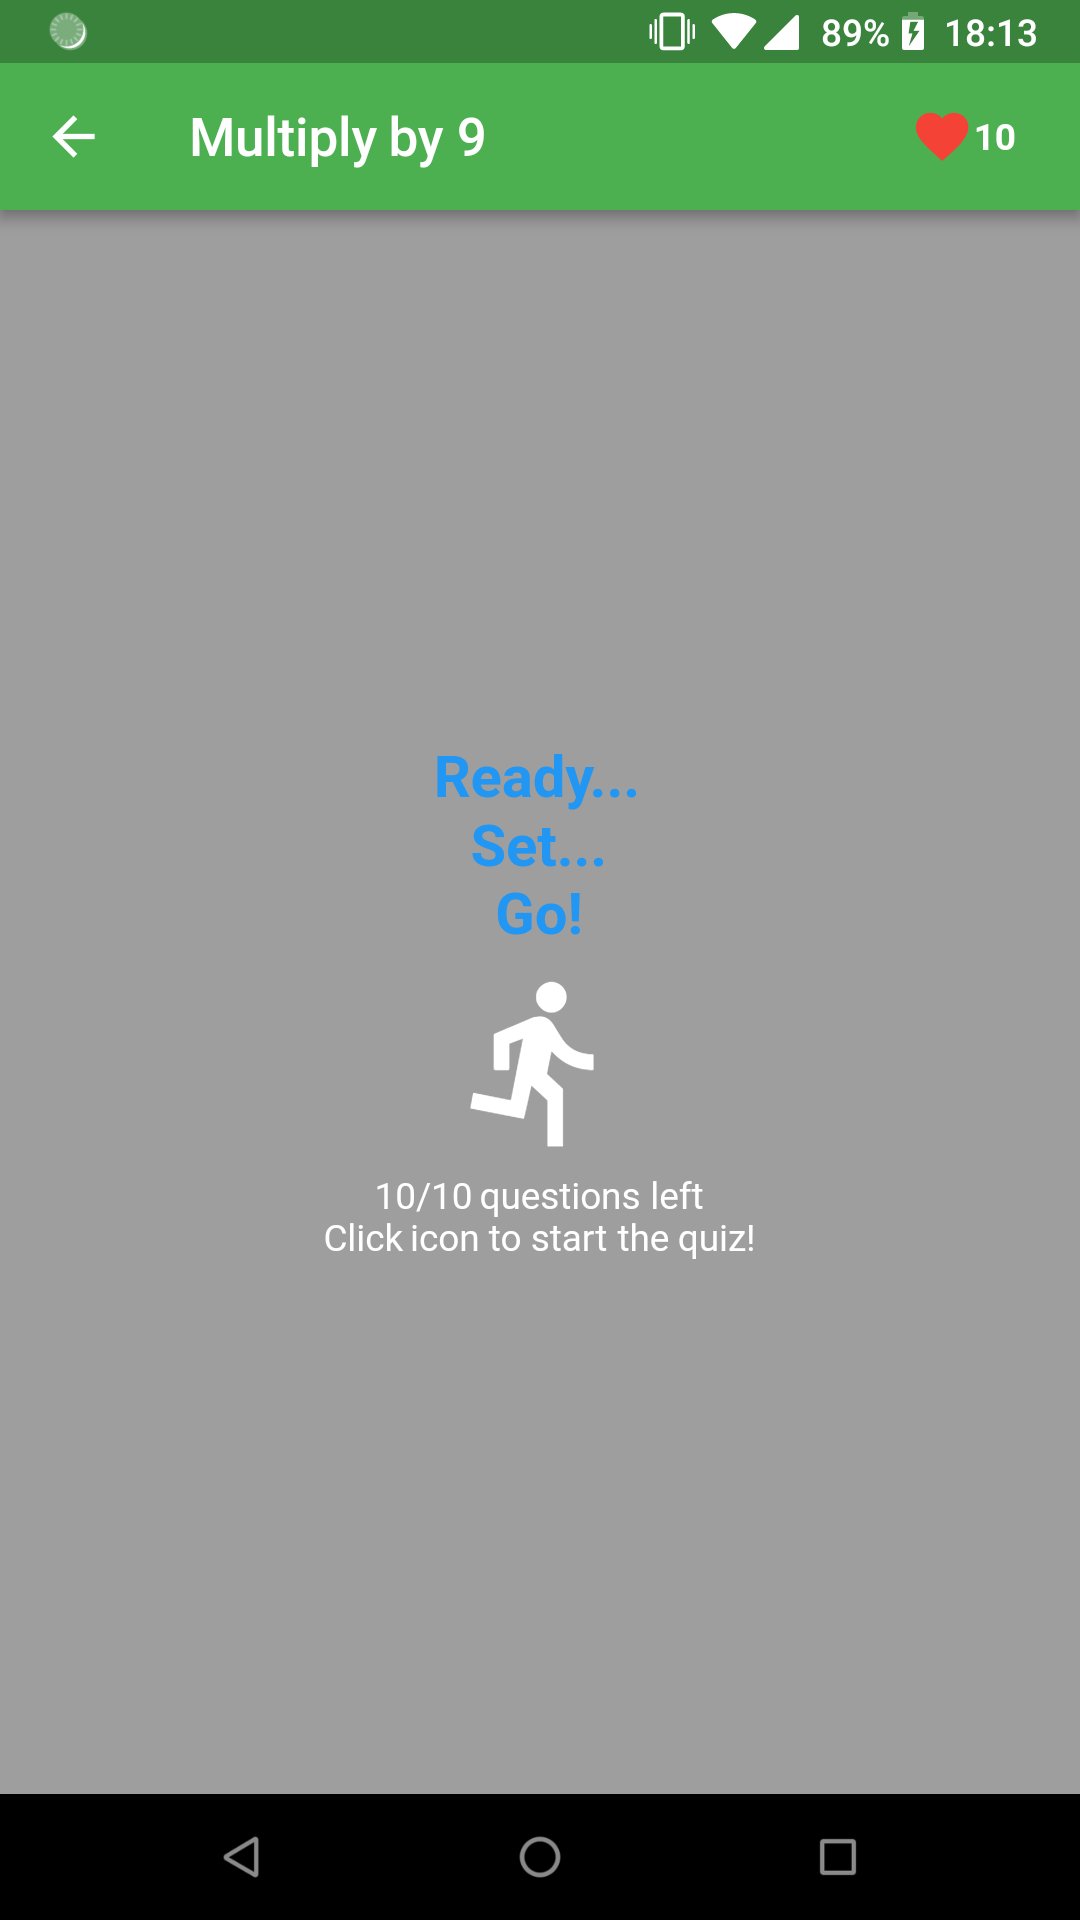
\includegraphics[width=.9\linewidth]{quiz-start}
  \caption{The quiz start page}
  \label{fig:quiz-start}
\end{subfigure}
\caption{The quiz related views}
\label{fig:quiz-views}
\end{figure}

\begin{figure}
\centering
\begin{subfigure}{.33\textwidth}
  \centering
  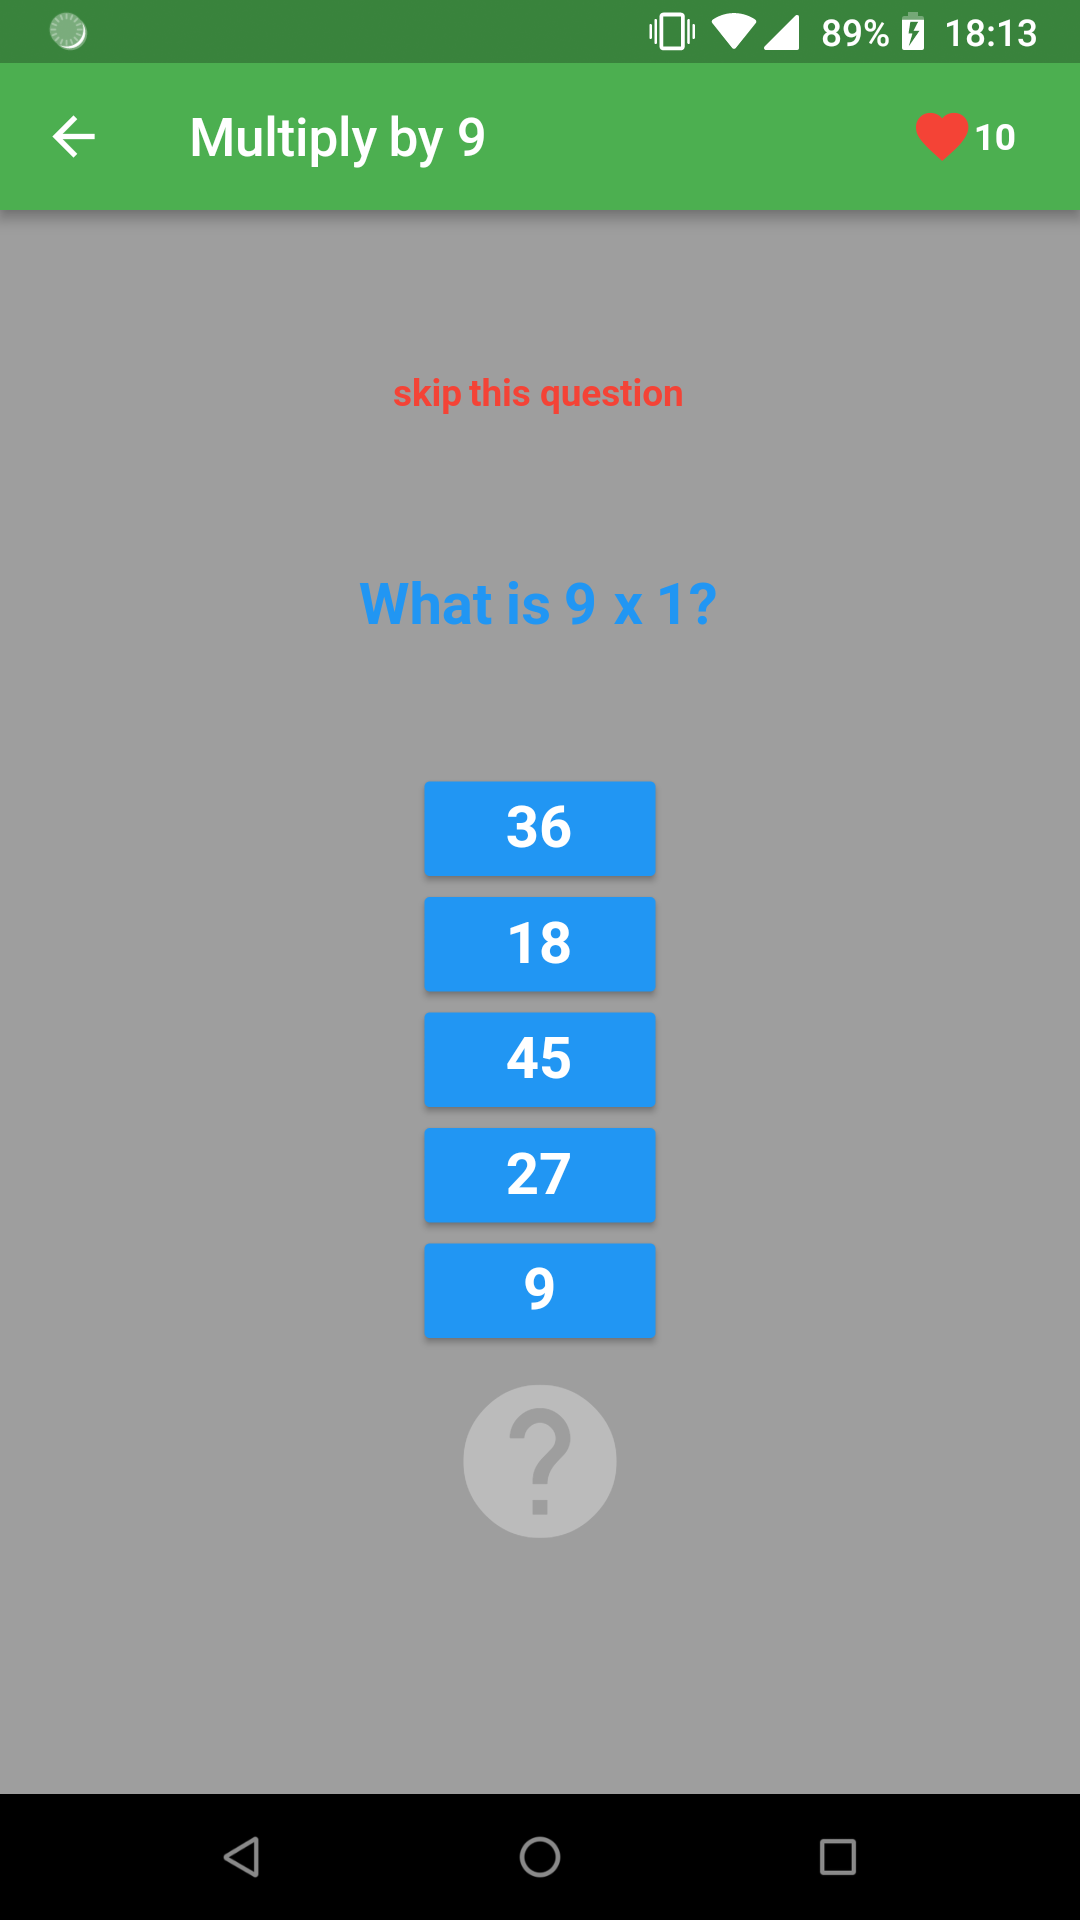
\includegraphics[width=.9\linewidth]{question}
  \caption{A question}
  \label{fig:question}
\end{subfigure}%
\begin{subfigure}{.33\textwidth}
  \centering
  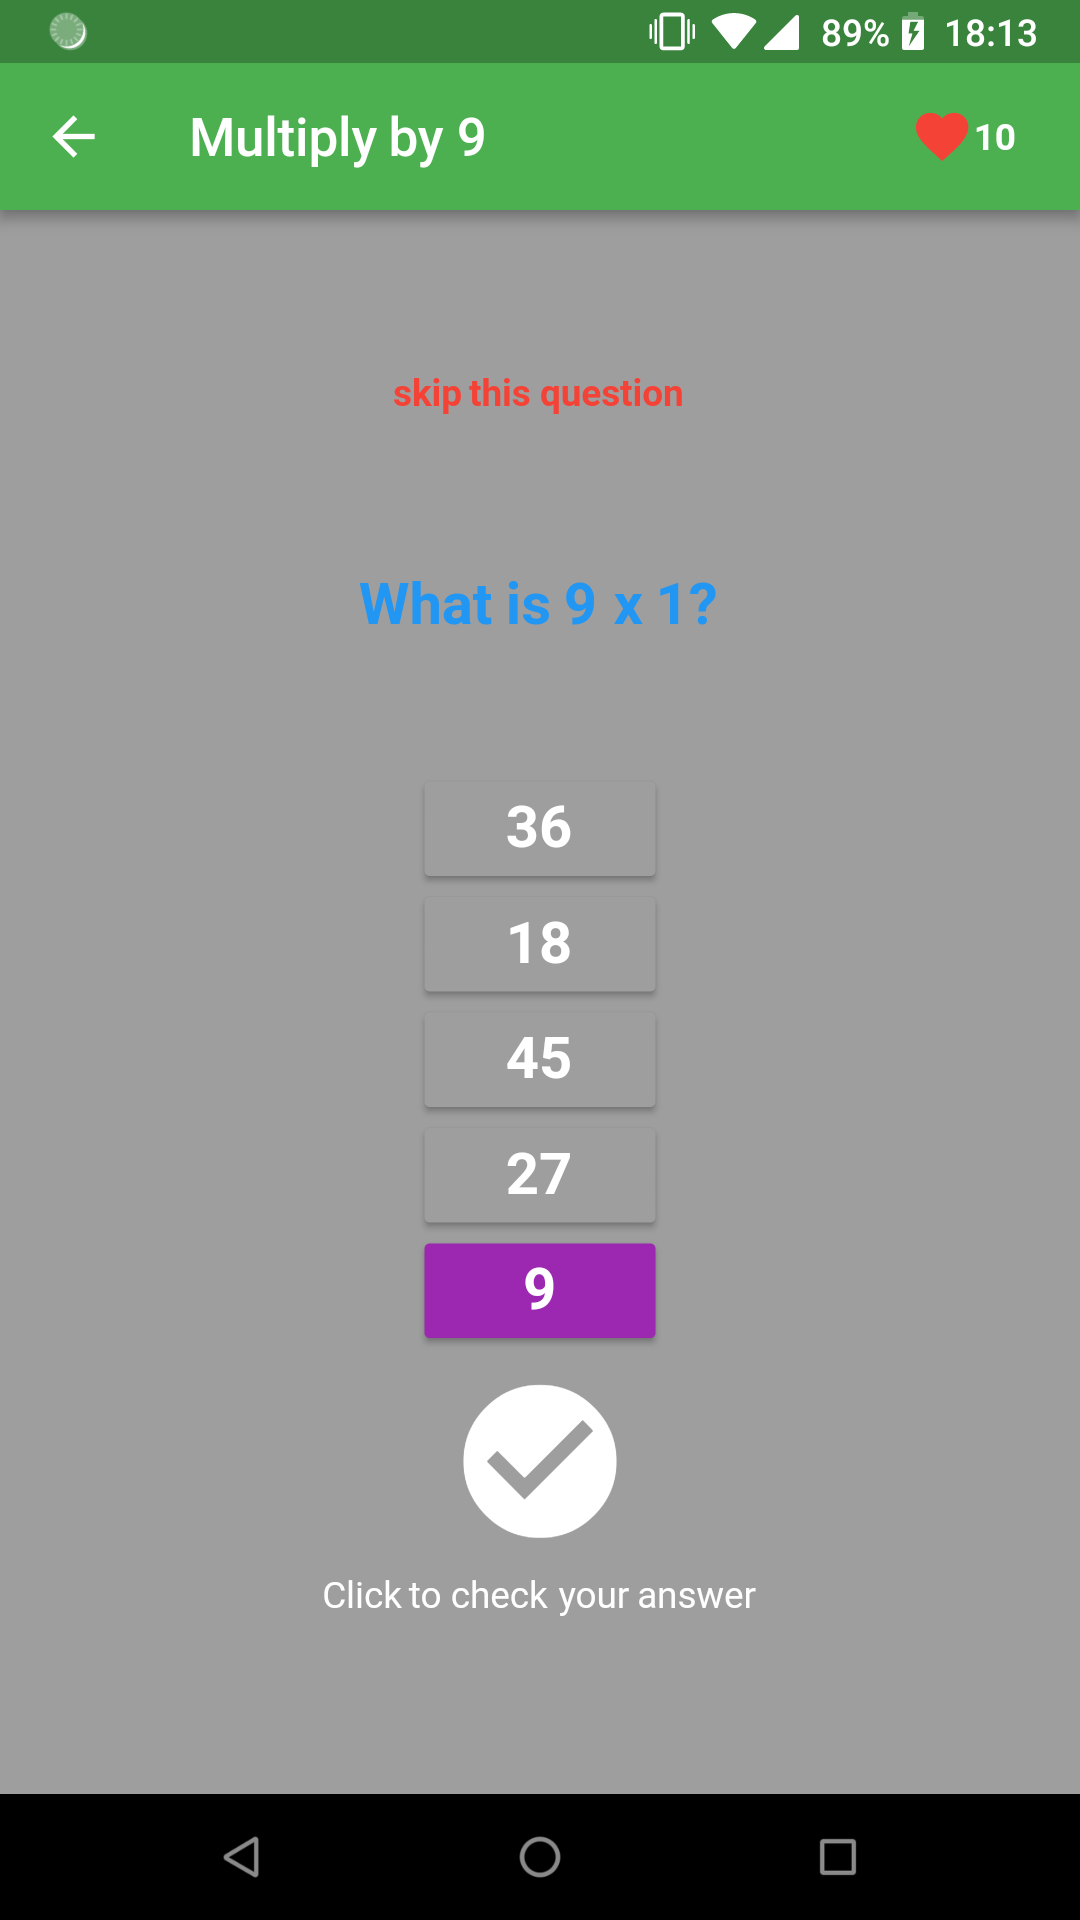
\includegraphics[width=.9\linewidth]{question-answered}
  \caption{The question answered}
  \label{fig:question-answered}
\end{subfigure}
\begin{subfigure}{.33\textwidth}
  \centering
  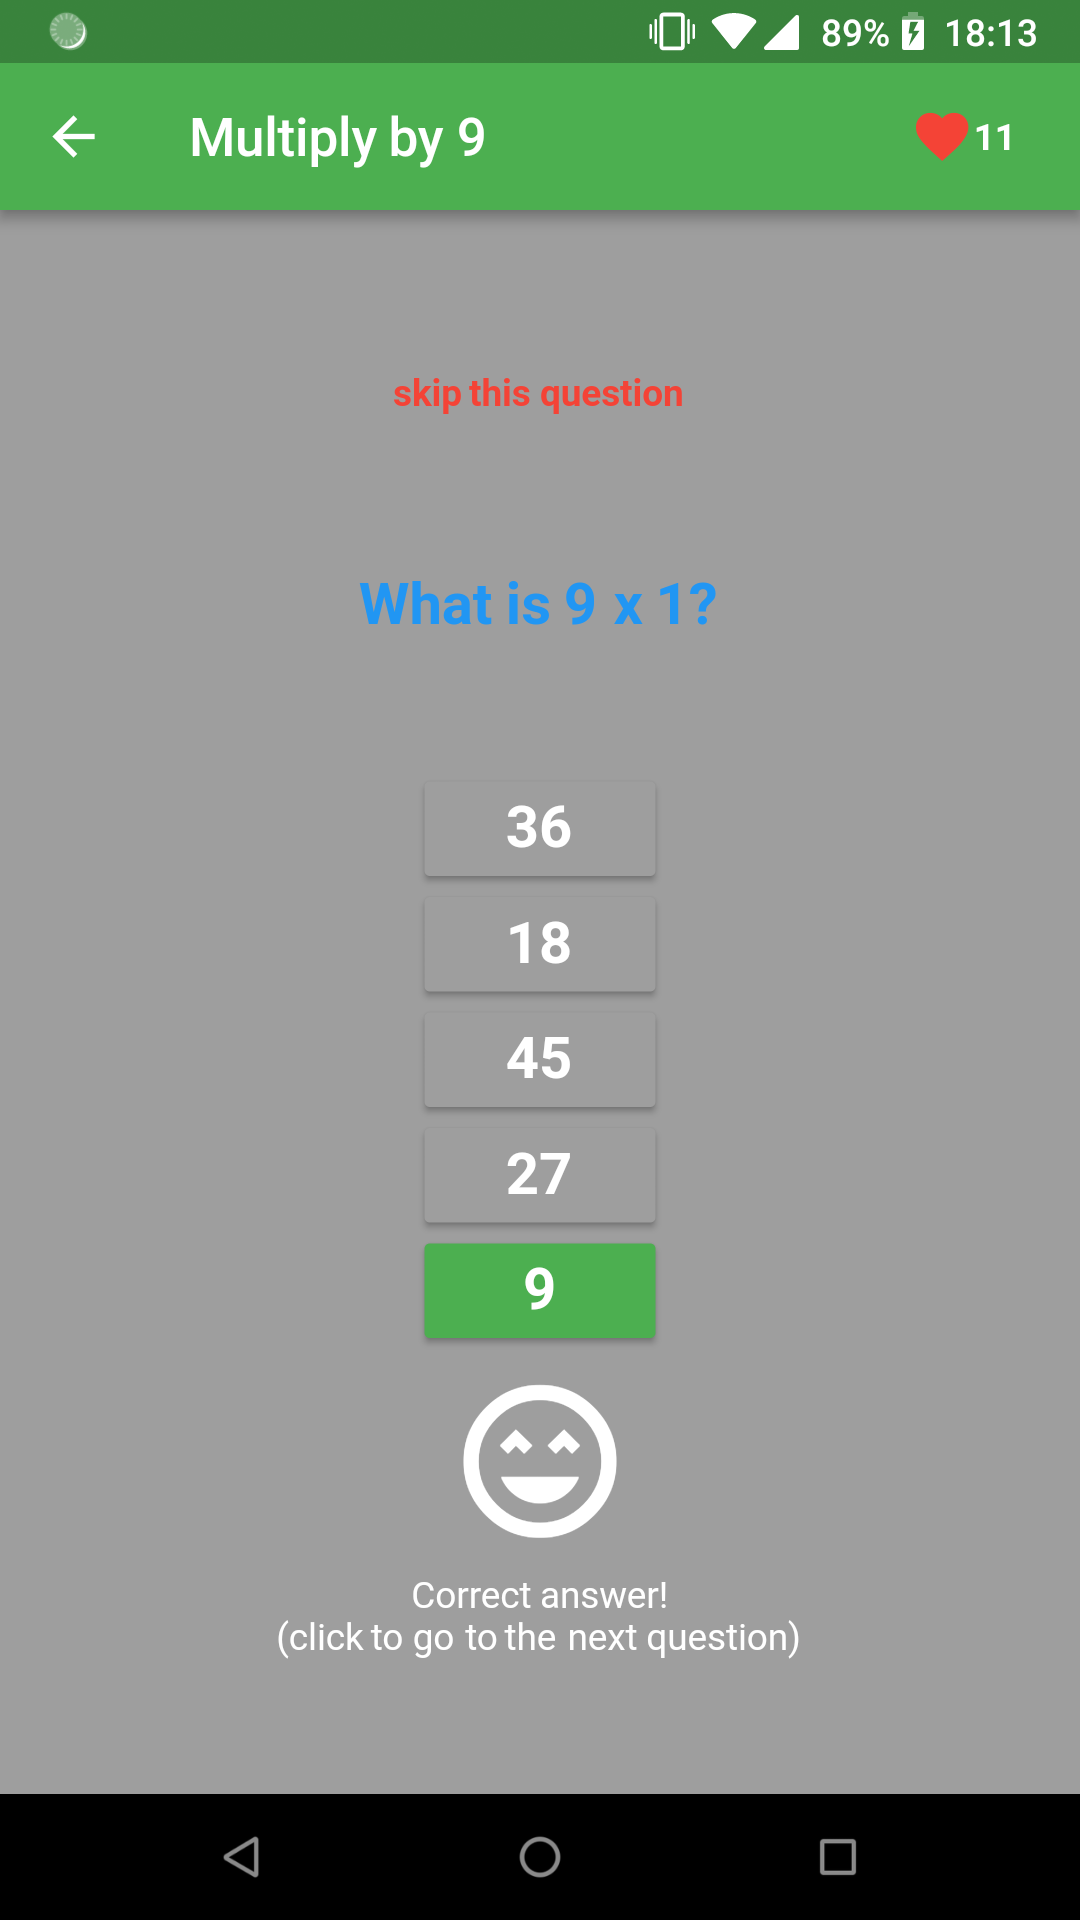
\includegraphics[width=.9\linewidth]{question-checked}
  \caption{The question checked}
  \label{fig:question-checked}
\end{subfigure}
\caption{The question view}
\label{fig:question-view}
\end{figure}

\begin{figure}
\centering
\begin{subfigure}{.33\textwidth}
  \centering
  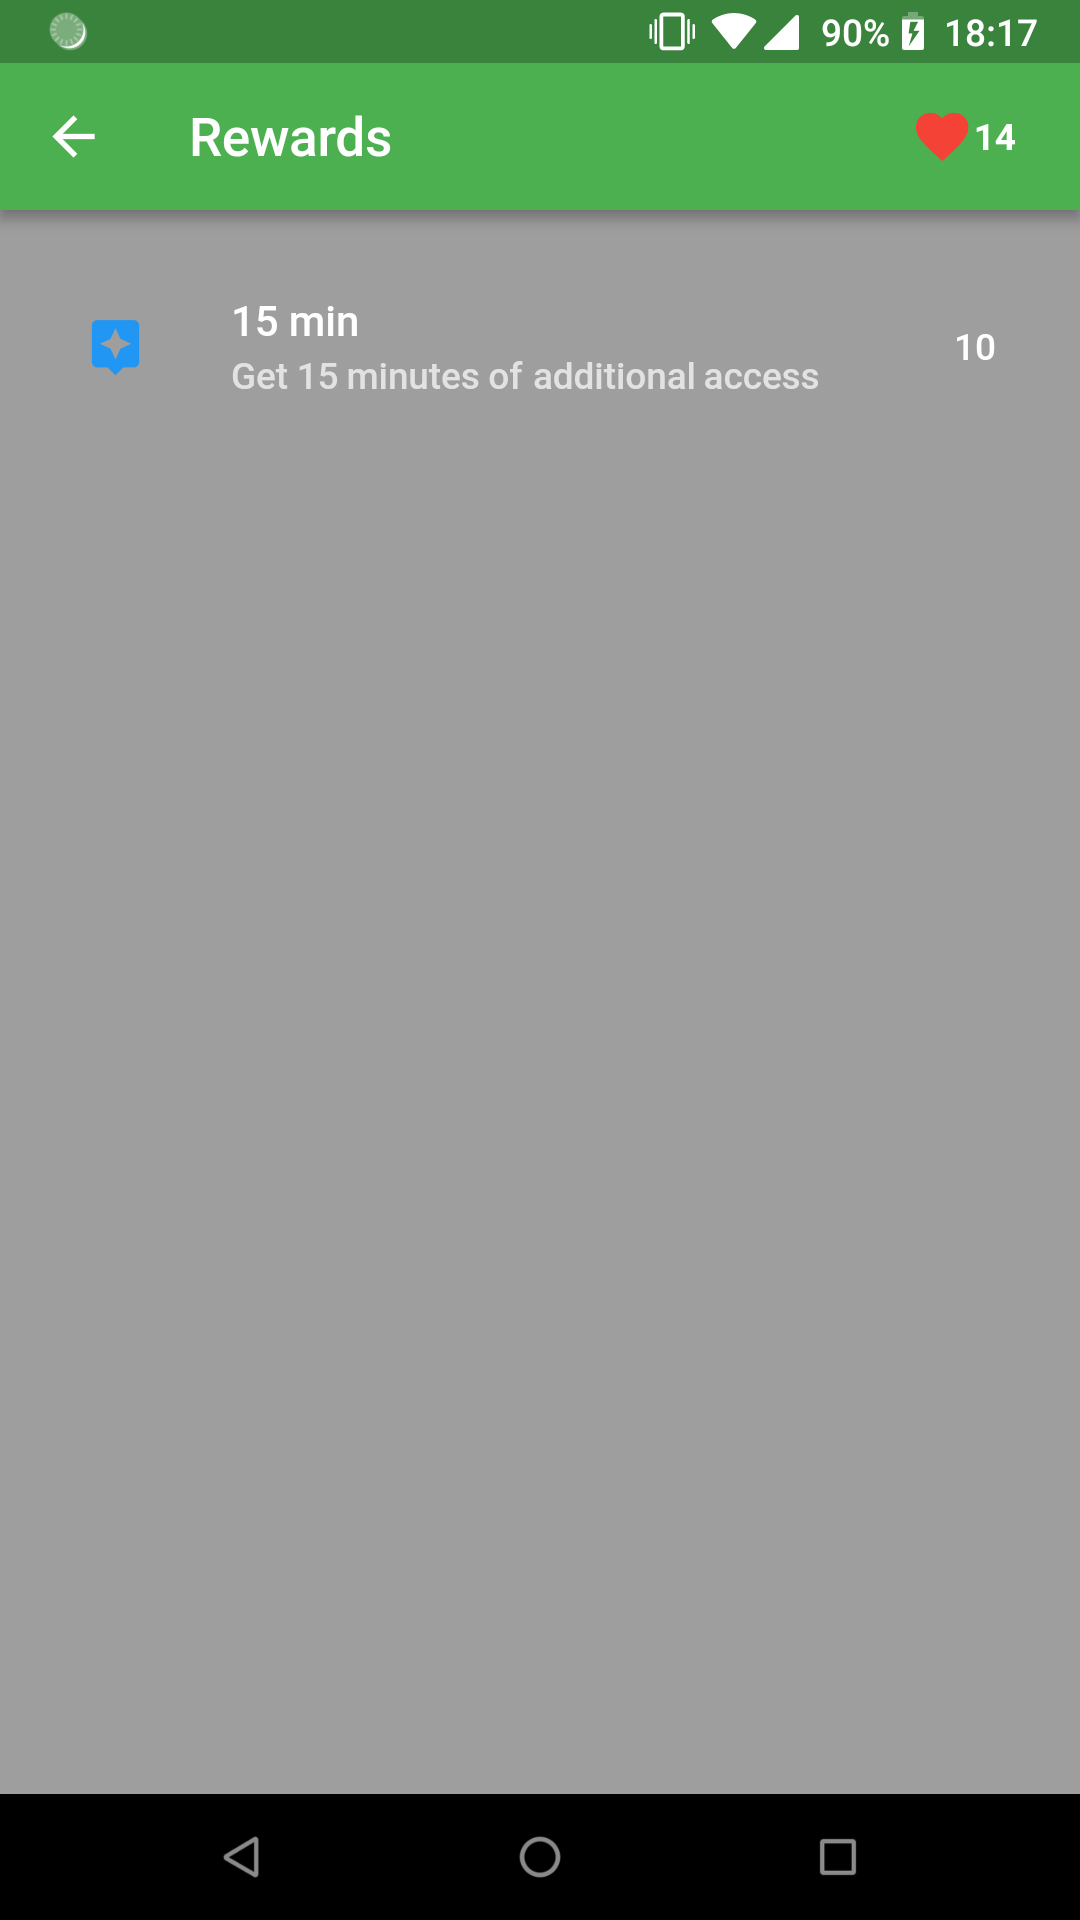
\includegraphics[width=.9\linewidth]{rewards}
  \caption{The rewards list view}
  \label{fig:rewards}
\end{subfigure}%
\begin{subfigure}{.33\textwidth}
  \centering
  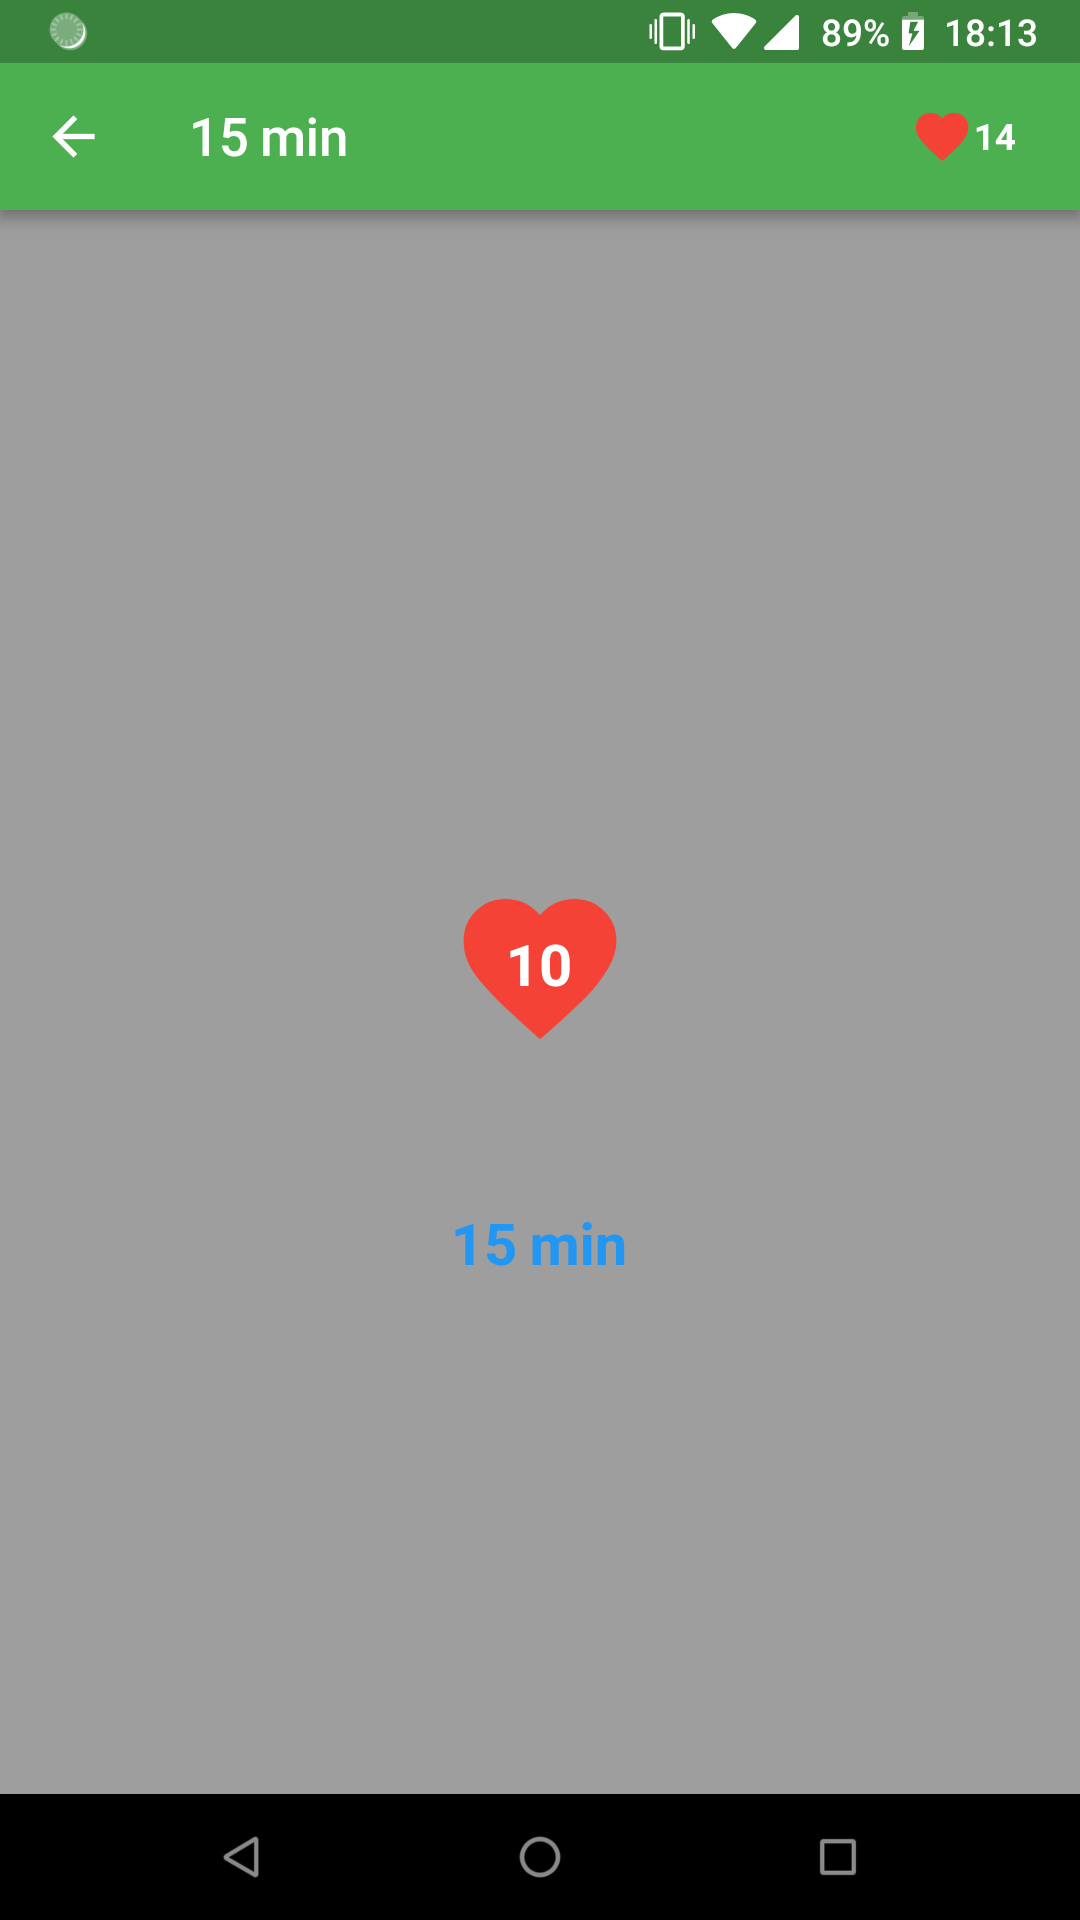
\includegraphics[width=.9\linewidth]{reward-get}
  \caption{Reward get view}
  \label{fig:reward-get}
\end{subfigure}
\begin{subfigure}{.33\textwidth}
  \centering
  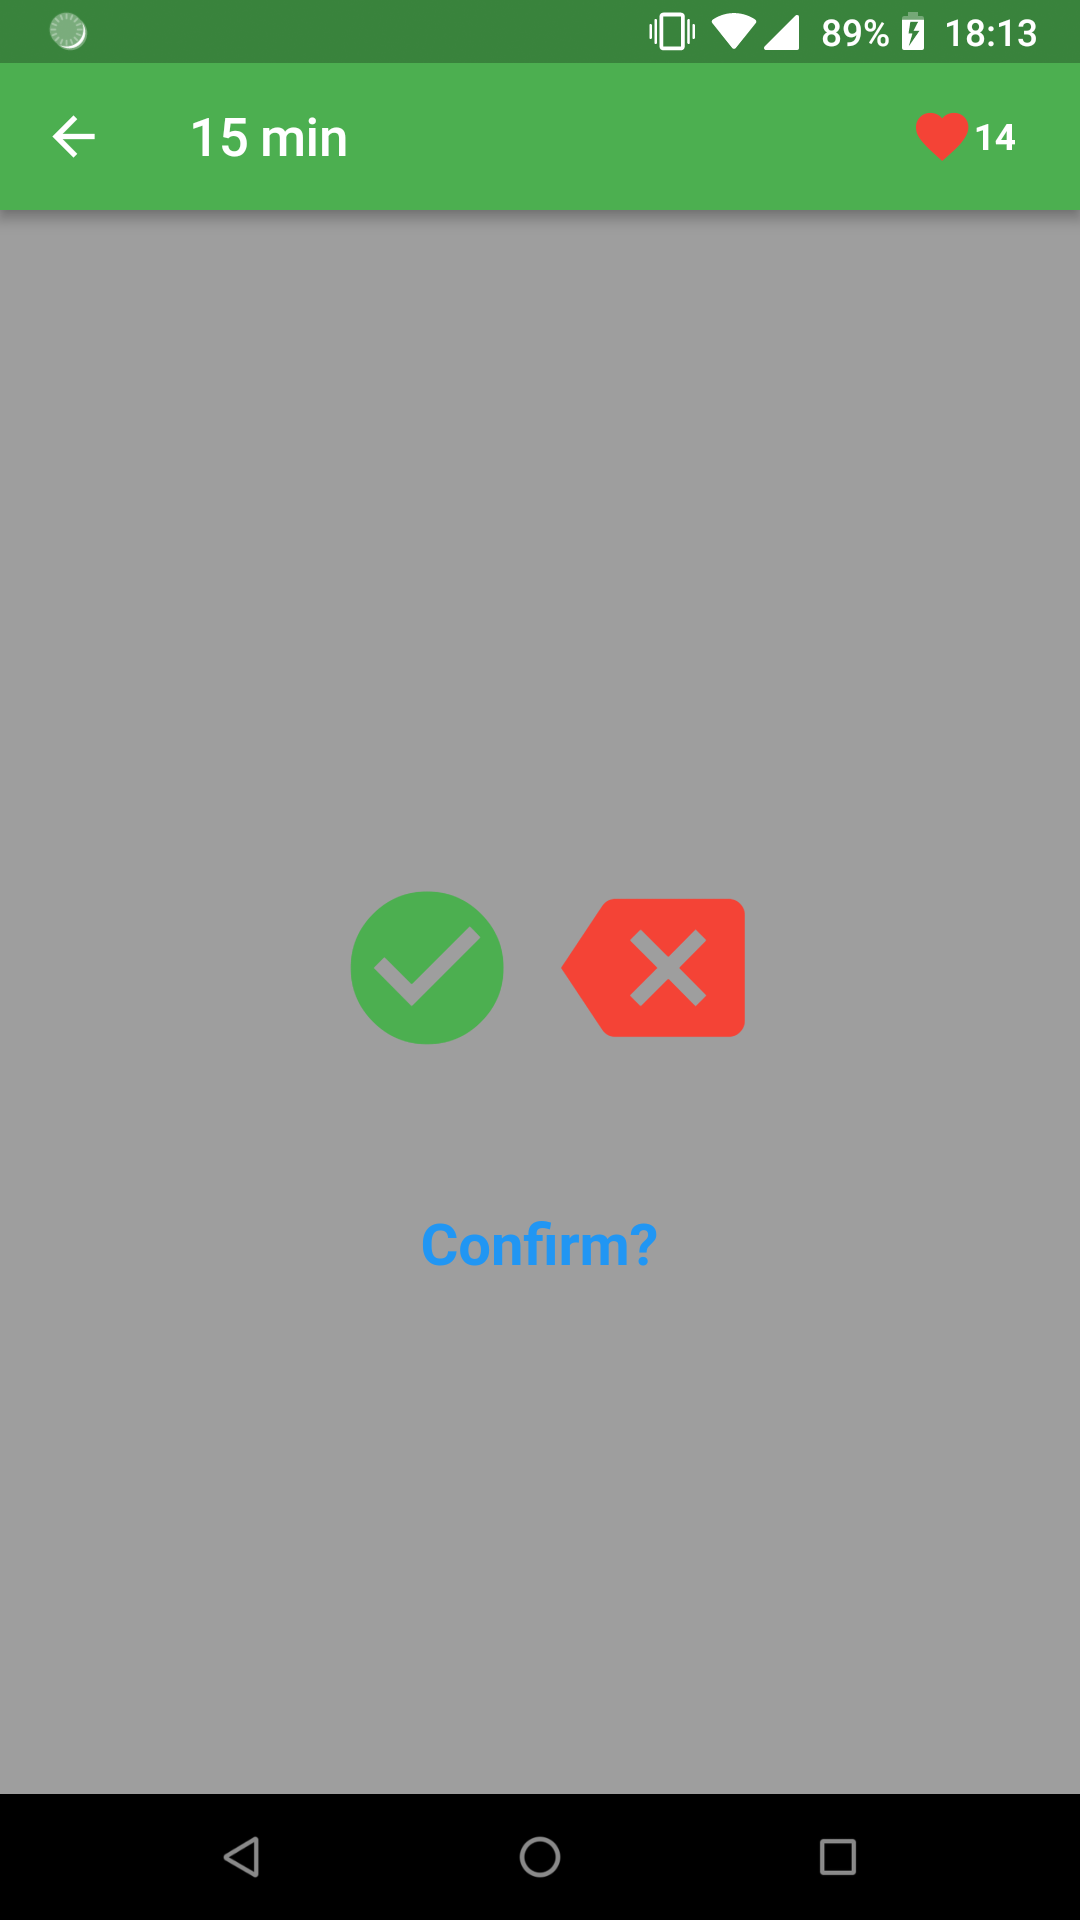
\includegraphics[width=.9\linewidth]{reward-confirm}
  \caption{Reward confirm view}
  \label{fig:reward-confirm}
\end{subfigure}
\caption{The reward views}
\label{fig:reward-views}
\end{figure}

%----------------------------------------------------------------------------------------